\chapter{What is the Parameter Space Like}
\label{chap:setting}

\begin{keypointsbox}
\noindent
\textbf{Key points (Chapter~\ref{chap:setting}).}
\begin{enumerate}\setlength{\itemsep}{2pt}
  \item \textbf{The dataset-restricted model map.}
  A Bayesian model induces a smooth map \(F_{\mathcal D}:\Theta \to \mathcal Z\) from parameters
  to dataset-restricted predictive quantities (e.g. logits or natural parameters). The fibres
  \(F_{\mathcal D}^{-1}(z)\) are precisely the sets of parameters that are indistinguishable on the dataset.

  \item \textbf{Local product structure on regular regions.}
  On regions where \(F_{\mathcal D}\) has constant rank, fibres are smooth submanifolds and the parameter
  space admits local coordinates in which it looks like a product
  \(\text{(prediction-changing)} \times \text{(prediction-preserving)}\).

  \item \textbf{Intrinsic splitting via an Ehresmann connection.}
  Choosing a horizontal complement to the vertical space \(\ker(dF_{\mathcal D})\) defines an Ehresmann
  connection, giving an intrinsic decomposition \(T_\theta\Theta = H_\theta \oplus V_\theta\) without relying
  on an embedded “image manifold”.

  \item \textbf{Why Bayes cares.}
  Posterior mass and uncertainty should respect this structure: vertical directions capture symmetries /
  non-identifiabilities, while horizontal directions control changes in predictions. This viewpoint clarifies
  how approximations (Laplace, VI) and samplers (MCMC) can be designed to move efficiently across fibres.
\end{enumerate}
\end{keypointsbox}

\begin{center}
\begin{minipage}{0.95\linewidth}
\noindent\textbf{Chapter \thechapter\ -- What is the Parameter Space Like:}\par\vspace{3pt}

\begin{tabular}{@{}p{0.83\linewidth}r@{}}
\hyperref[sec:informal_local_product]{\thechapter.2\;\;Informal picture: parameter space as a local product space} \dotfill & \pageref{sec:informal_local_product}\\
\hyperref[sec:parammanifold_formal]{\thechapter.3\;\;Formal picture: parameter manifold and bundle viewpoint} \dotfill & \pageref{subsec:parammanifold_formal}\\
\hyperref[sec:sowhat]{\thechapter.4\;\;So what? Geometric quantities and why we care} \dotfill & \pageref{sec:sowhat}\\
\end{tabular}
\end{minipage}
\end{center}



\noindent
This chapter builds the geometric foundation used throughout the thesis. The guiding idea is that,
for a fixed dataset \(\mathcal D\), a model is best understood through the dataset-restricted \emph{forward map}
\(F_{\mathcal D}:\Theta \to \mathcal Z\) that sends parameters to predictive quantities (e.g. logits).
Parameters that produce identical predictions on \(\mathcal D\) lie on the same \emph{fibre}
\(F_{\mathcal D}^{-1}(z)\), and these fibres capture the model's continuous reparameterizations.

Under mild regularity conditions, the parameter space admits a \emph{local product} structure: a decomposition of the parameter space into directions that change predictions and directions that move within fibres. The upshot of this construction is that Bayesian computation takes place on a parameter space that is not Euclidean, but instead carries a geometry explicitly accounting for \emph{reparameterizations} of the forward map—here, a neural network

We begin with an informal treatment anchored in the linear-Gaussian case, where the decomposition is global and explicit, and provide an intuitive description of what the parameter space looks like. This is followed by a more rigorous formal treatment where we formalize the intuitive descriptions to describe the parameter space as a Riemannian manifold. Finally, we briefly discuss the consequences of this construction and foreshadow the rest of the thesis.


\section{Informal picture: Parameter Space as a local product space} 
\label{sec:informal_local_product}

\subsection{Global product space in the linear--Gaussian case}
\label{subsec:linear_gaussian_global_product}

To build intuition on the geometry of the parameter space without any differential geometry, we begin with Bayesian Linear Regression with a Gaussian prior and a Gaussian likelihood. In this model, the parameter space has a global product structure: there is a whole subspace of directions that do not change the dataset-restricted predictions at all.

\paragraph{Model and the dataset-restricted map.}
Let $\theta\in\Theta=\mathbb{R}^P$. Consider a linear forward map
\[
  f_\theta(x) \;=\; x^\top \theta \in \mathbb{R}.
\]
Given a supervised dataset $\mathcal{D}=\{(x^{(n)},y^{(n)})\}_{n=1}^N$, stack the inputs into the design matrix
$X\in\mathbb{R}^{N\times P}$ with rows $(x^{(n)})^\top$, and stack labels into $Y\in\mathbb{R}^N$. We are interested in the setting where $X$ is low-rank, i.e. it has zero singular values. A sufficient condition for this is when $N < P$, so the analysis below is especially relevant for \emph{overparameterized models}.
The dataset-restricted prediction map is
\[
  F_{\mathcal{D}}(\theta)
  \;:=\;
  \begin{bmatrix}
    f_\theta(x^{(1)})\\ \vdots\\ f_\theta(x^{(N)})
  \end{bmatrix}
  \;=\; X\theta \in \mathbb{R}^N.
\]
We have the following likelihood and prior models:
\[
\underbrace{
Y \mid \theta \sim \mathcal{N}(X\theta,\sigma^2 I)
}_{\scriptstyle \text{likelihood}}
\qquad
\underbrace{
\theta \sim \mathcal{N}(0,\tau^2 I)
}_{\scriptstyle \text{prior}}
\]

\paragraph{Fibres are affine subspaces}
Two parameters $\theta,\theta'$ are indistinguishable on the dataset iff $X\theta=X\theta'$,
i.e.\ iff $X(\theta-\theta')=0$. So the fibre through $\theta$ is
\[
  F_{\mathcal{D}}^{-1}(\theta)
  \;=\;
  \theta + \ker(X).
\]
Moving inside $\ker(X)$ does not change the logits/predictions on the dataset.
Geometrically, parameter space is foliated by parallel affine subspaces.

\paragraph{A global splitting: prediction-changing vs prediction-preserving.}
Because $F_{\mathcal{D}}$ is a linear map, there is a global, dataset-dependent decomposition of parameter space into the kernel subspace and a co-image subspace:
\[
  \mathbb{R}^P
  \;=\;
  \underbrace{\ker(X)}_{\text{prediction-preserving}}
  \;\oplus\;
  \underbrace{\mathrm{im}(X^\top)}_{\text{prediction-changing (row space)}}.
\]
This follows from the rank-nullity theorem. Every $\theta$ can be uniquely written as
\[
  \theta = \theta_{\parallel} + \theta_{\perp},
  \qquad
  \theta_{\parallel}\in \mathrm{im}(X^\top),\;\; \theta_{\perp}\in \ker(X),
\]
and crucially
\[
  X\theta = X\theta_{\parallel}
  \quad\text{(the dataset predictions ignore }\theta_{\perp}\text{ entirely).}
\]


\begin{figure}[ht]
\centering
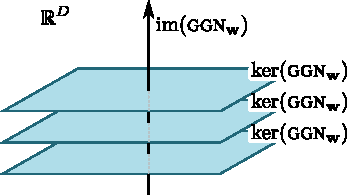
\includegraphics[width=0.6\linewidth]{chapters/ch3_figures/linear_kernel.pdf}
\caption{The weight space can be decomposed into directions of \emph{reparameterizations} and \emph{functional changes}. For linear models, these are linear subspaces given by the kernel and the image, respectively.\looseness=-1}
\label{fig:stacked_kernels}
\end{figure}


\paragraph{Posterior factorization}
In this model, the posterior is exactly Gaussian,
\[
  p(\theta\mid \mathcal{D})
  \;=\;
  \mathcal{N}\!\bigl(\theta \,;\, \mu,\Sigma\bigr),
  \qquad
  \Sigma^{-1} = \tau^{-2}I + \sigma^{-2}X^\top X,
  \qquad
  \mu = \sigma^{-2}\Sigma X^\top y.
\]

The decomposition of the parameter space also has a profound effect on the posterior: It can also be decomposed into these two subspaces. 

Given our assumption that $X$ is low-rank, $X^\top X$ admits an eigendecomposition, with eigenvectors $\mathbf{U_1}$ and $\mathbf{U_2}$ corresponding to non-zero and zero eigenvalues, respectively. Then the posterior covariance is given by: 

\begin{align}
\Sigma
&=\Bigg(
\sigma^{-2}
\left[\begin{array}{c}
\mathbf{U}_1^{\top}\\ \hline \mathbf{U}_2^{\top}
\end{array}\right]
\left[\begin{array}{c|c}
\tilde{\mathbf{\Lambda}} & \mathbf{0}\\ \hline
\mathbf{0} & \mathbf{0}
\end{array}\right]
\left[\begin{array}{c}
\mathbf{U}_1\\ \hline \mathbf{U}_2
\end{array}\right]
\;+\;\tau^{-2}\mathbf{I}
\Bigg)^{-1} \nonumber\\
&=
\mathbf{U}_1\big(\sigma^{-2}\tilde{\mathbf{\Lambda}}+\tau^{-2}\mathbf{I}_r\big)^{-1}\mathbf{U}_1^{\top}
\;+\;
\tau^{2}\,\mathbf{U}_2\mathbf{U}_2^{\top}.
\end{align}



Moreover, since $X^\top y\in\mathrm{im}(X^\top)=\mathrm{span}(\mathbf U_1)$, the posterior mean has no $\mathbf U_2$
component:
\[
\mu=\sigma^{-2}\Sigma X^\top y
=
\mathbf{U_1} m_1,
\qquad
m_1:=\sigma^{-2}(\tilde{\mathbf{\Lambda}}+\alpha \mathbf I_r)^{-1}\mathbf{U_1}^\top X^\top y,
\qquad
\mathbf U_2^\top \mu=0.
\]

We can then write the posterior as the sum of two independent random variables i.e. $\theta | \mathcal{D} \overset{d}{=} \theta_{\textrm{im}} + \theta_{\textrm{ker}}$, corresponding to the posterior projected onto the prediction-changing subspace and the prior projected onto the  prediction-preserving subspace, respectively: 
\begin{align}
    &\theta_{\textrm{im}}\mid\mathcal D\sim\mathcal{N}(\mu,\;\mathbf{U_1}(\tilde{\mathbf{\Lambda}}+\alpha \mathbf I_r)^{-1}\mathbf{U_1}^\top),
\qquad
\theta_{\textrm{ker}}\mid\mathcal D\sim\mathcal{N}(\mathbf{0},\;\alpha^{-1}\mathbf{U_2}\mathbf{U_2}^\top),
\\
&\theta_{\textrm{im}} \perp\ \theta_{\textrm{ker}}
\end{align}

\todo{Add illustration of this}

\paragraph{Prediction under the decomposed posterior}
For any integrable test function $\varphi:\mathbb{R}^P\to\mathbb{R}$
\begin{align}
    \mathbb{E}[\varphi(\theta)\mid\mathcal D] 
    &= \iint \varphi(\theta_{\textrm{im}} + \theta_{\textrm{ker}})\,p(\theta_{\textrm{im}}\mid\mathcal D)\,
    p(\theta_{\textrm{ker}})\;d\theta_{\textrm{im}}\,d\theta_{\textrm{ker}} \\
    &= \int \Bigg[ \int \varphi(\theta_{\textrm{im}} + \theta_{\textrm{ker}})\,p(\theta_{\textrm{ker}})\;d\theta_{\textrm{ker}} \Bigg]\,
    p(\theta_{\textrm{im}}\mid\mathcal D)\;d\theta_{\textrm{im}}
    \qquad \text{(Fubini--Tonelli)}.
\end{align}

If this test function happens to be the likelihood of a new observation then the integral above represents Bayesian model averaging. Thus the decomposition of the parameter space affects both Bayesian inference and prediction.
\subsection{From global to local: Taylor's theorem and the local product space}
\label{subsec:local_linearization_product}

In the Linear--Gaussian case, the parameter space has a simple geometry: it is a global product of two subspaces. For neural networks, the map $F_{\mathcal{D}}$ is nonlinear, so we cannot expect such a global product structure. However, under mild regularity conditions, \emph{locally, the model map is a linear function}. A lot of the analysis above still holds, but only locally. The parameter space looks like a product of fibre directions and prediction-changing directions, but these directions also change within the parameter space.

\paragraph{The dataset-restricted model map}
Fix a dataset \(\mathcal D=\{(x^{(n)},y^{(n)})\}_{n=1}^N\).
Recall that the dataset-restricted prediction map
\begin{equation}
  F_{\mathcal D}:\Theta\to\mathcal U^N,
  \qquad
  F_{\mathcal D}(\theta)
  \;:=\;
  \bigl(f_\theta(x^{(1)}),\dots,f_\theta(x^{(N)})\bigr),
  \label{eq:dataset_restricted_map_local}
\end{equation}
so that the likelihood factors through \(F_{\mathcal D}\):
\[
  p(\mathcal D\mid \theta)
  \;=\;
  \prod_{n=1}^N p\bigl(y^{(n)}\mid f_\theta(x^{(n)})\bigr)
  \;=\;
  \mathcal{L}\,\bigl(F_{\mathcal D}(\theta)\bigr)
\]
for a suitable function \(\mathcal{L}:\mathcal U^N\to\mathbb{R}_+\).
As before, the \emph{fibres} are the dataset-identifiability classes
\(
\mathcal F_z := F_{\mathcal D}^{-1}(z)
\),
i.e.\ the sets of parameters that agree on all training inputs.

\paragraph{Local Linear Approximation}

We stack the per-datum Jacobians of the model into $J_{\mathcal{D}}(\theta) = [\frac{\partial f_\theta(x^{(1)})}{\partial \theta}; \ldots; [\frac{\partial f_\theta(x^{(N)})}{\partial \theta}] \in \mathbb{R}^{NO \times D}$. Then under mild regularity conditions, for any \(\theta_0\in\Theta\) and \(\theta=\theta_0+\delta\).
By Taylor's theorem,
\begin{equation}
  F_{\mathcal D}(\theta_0+\delta)
  \;=\;
  F_{\mathcal D}(\theta_0)
  \;+\;
  J_{\mathcal D}(\theta_0)\,\delta
  \;+\;
  R_{\theta_0}(\delta),
  \label{eq:taylor_F}
\end{equation}
where \(J_{\mathcal D}(\theta_0)=dF_{\mathcal D}(\theta_0)\) is the stacked Jacobian, and the remainder satisfies
\[
  \|R_{\theta_0}(\delta)\|
  \;\le\;
  C_{\theta_0}\,\|\delta\|^2
  \qquad \text{for all }\|\delta\|\le \varepsilon
\]
for some constant \(C_{\theta_0}\) depending on second-derivative bounds of \(F_{\mathcal D}\) on the ball
\(B(\theta_0,\varepsilon)\).

\paragraph{Are we even allowed to do this?}
It might seem like linearizing the model is a brutal approximation valid only infinitesimally. However, we can show that global Bayesian computations are well-approximated by patching together these local linearizations.
For some $\theta_0$, define the linearized map $\widetilde F_{\theta_0}(\theta):=F_{\mathcal D}(\theta_0)+J_{\mathcal D}(\theta_0)(\theta-\theta_0)$.
We define the local linearized likelihood and posterior approximation as:
\begin{align}
    \widetilde{\mathcal L}_{\theta_0}(\theta):=\mathcal L\,\bigl(\widetilde F_{\theta_0}(\theta)\bigr),
\qquad
\widetilde p_{\theta_0}(\theta\mid\mathcal D)\propto p(\theta)\,\widetilde{\mathcal L}_{\theta_0}(\theta).
\end{align}

Consider a ball $B(\theta_0,\varepsilon)$. Taylor's theorem guarantees a bound on the mapping error $\|F_{\mathcal D}(\theta)-\widetilde F_{\theta_0}(\theta)\|\le C_{\theta_0}\|\theta-\theta_0\|^2$.
We \textbf{assume} that the log-likelihood $\log\mathcal L$ is locally Lipschitz continuous.
This implies there exists a constant $L_{\theta_0}$ such that for all $\theta\in B(\theta_0,\varepsilon)$,
\begin{equation}
\label{eq:loglik_bound_ball}
\bigl|\log \mathcal L(F_{\mathcal D}(\theta))-\log \widetilde{\mathcal L}_{\theta_0}(\theta)\bigr|
\;\le\; L_{\theta_0}C_{\theta_0}\,\|\theta-\theta_0\|^2
\;\le\; \eta,
\end{equation}
where we choose $\varepsilon$ small enough such that $\eta$ is a small error tolerance.
Exponentiating this yields a bound on the likelihood ratio:
\begin{equation}
\label{eq:lik_ratio_ball}
e^{-\eta}\;\le\;\frac{\mathcal L(F_{\mathcal D}(\theta))}{\widetilde{\mathcal L}_{\theta_0}(\theta)}\;\le\;e^{\eta}.
\end{equation}

Thus, locally, the likelihood is bounded by the linearized model. To extend this to the \emph{global} posterior, we patch these local approximations together.
We \textbf{assume} parameter space $\Theta$ is paracompact (such as if it is euclidean or a manifold), it admits a locally finite open cover by such balls $\Theta \subset \cup_{i} B(\theta_i, \varepsilon_i)$ where the bound \eqref{eq:lik_ratio_ball} holds on each ball.
Let $\{\psi_i\}$ be a smooth partition of unity subordinate to this cover, meaning $\psi_i:\Theta\to[0,1]$ such that:
\begin{align}
    \mathrm{supp}(\psi_i)\subset B_i, \ \textrm{and} \ \sum_{i} \psi_i(\theta)=1 \quad \forall \theta \in \Theta.
\end{align}

Let $\pi(\theta):=p(\theta)\,\mathcal L(F_{\mathcal D}(\theta))$ be the true unnormalized posterior. On each patch $B_i$,
we denote the local linearized surrogate as $\widetilde\pi_i(\theta):=p(\theta)\,\mathcal L(\widetilde F_i(\theta))$.
Because the partition of unity sums to one, we can define a \emph{global surrogate posterior} $\widehat{\pi}(\theta)$ as the weighted average of these local linear models:
\begin{align}
    \widehat\pi(\theta)\;:=\;\sum_{i} \psi_i(\theta)\,\widetilde\pi_i(\theta),
\qquad \theta\in \Theta.
\end{align}
By multiplying the local bound \eqref{eq:lik_ratio_ball} by $\psi_i(\theta)$ and summing over all $i$, we derive a \emph{global} pointwise bound on the unnormalized densities:
\begin{equation}
\label{eq:patched_ratio}
e^{-\eta}\,\widehat\pi(\theta)\;\le\;\pi(\theta)\;\le\;e^{\eta}\,\widehat\pi(\theta),
\qquad \forall\,\theta\in \Theta.
\end{equation}

This also gives us a bound on the model evidence. Let $Z:=\int_\Theta \pi(\theta)\,d\theta$ and $\widehat Z:=\int_\Theta \widehat\pi(\theta)\,d\theta$. Assuming the posterior is normalizable ($Z < \infty$), integrating \eqref{eq:patched_ratio} yields $e^{-\eta}\widehat Z\le Z\le e^{\eta}\widehat Z$.
We define the normalized global posteriors as:
\begin{align}
    p(\theta\mid\mathcal D):=\frac{\pi(\theta)}{Z},
    \qquad
\widehat p(\theta\mid\mathcal D):=\frac{\widehat\pi(\theta)}{\widehat Z}.
\end{align}

Combining the bounds on $\pi$ and $Z$ implies that the ratio of the true to the surrogate posterior is bounded by $e^{2\eta}$. This yields a bound on the Total Variation (TV) distance:
\begin{align}
    \mathrm{TV}(p,\widehat p)
\;\le\;\frac{e^{2\eta}-1}{e^{2\eta}+1}
\end{align}
Furthermore, for any bounded measurable test function $\varphi$ (such as a the predictive function),
\begin{align}
    \bigl|\mathbb E_{p}[\varphi(\theta)]-\mathbb E_{\widehat p}[\varphi(\theta)]\bigr|
\;\le\;2\|\varphi\|_\infty\,\frac{e^{2\eta}-1}{e^{2\eta}+1}
\end{align}

In particular, for any new input $x_\star$,
letting $\varphi(\theta)=P(y \mid x_\star,\theta)$ gives a guarantee on the predictive error:

\textcolor{blue}{TODO}

This confirms that the global nonlinear posterior is well-approximated by the collection of local linear fibres.
\paragraph{Local product structure.}
At $\theta_0$, the linearized map $\delta\mapsto J_{\mathcal D}(\theta_0)\delta$ plays the role of the design matrix in the
linear--Gaussian example. In particular, the \emph{infinitesimal fibre (prediction-preserving) directions} are
\begin{align}
    V_{\theta_0}\;:=\;\ker\!\bigl(dF_{\mathcal D}(\theta_0)\bigr)\;=\;\ker\!\bigl(J_{\mathcal D}(\theta_0)\bigr),
\end{align}

since $J_{\mathcal D}(\theta_0)\delta=0$ implies $F_{\mathcal D}(\theta_0+\delta)=F_{\mathcal D}(\theta_0)+O(\|\delta\|^2)$.
We can also choose an orthogonal subspace $H_{\theta_0}$ corresponding to prediction-changing subspace. In the language of differential geometry the open cover will correspond to the charts, and the direct sum of subspaces $H_{\theta_0}\oplus V_{\theta_0}$ will correspond to the tangent space at each parameter
\begin{align}
    T_{\theta_0}\Theta \;\cong\; H_{\theta_0}\oplus V_{\theta_0}
\end{align}
A canonical choice is
$H_{\theta_0}=V_{\theta_0}^\perp=\mathrm{im}(J_{\mathcal D}(\theta_0)^\top)$, yielding the pointwise split
\[
T_{\theta_0}\Theta \;=\; \ker(J_{\mathcal D}(\theta_0))\ \oplus\ \mathrm{im}(J_{\mathcal D}(\theta_0)^\top).
\]
Unlike the linear model, $J_{\mathcal D}(\theta)$ depends on $\theta$, so the subspaces
$V_\theta=\ker(J_{\mathcal D}(\theta))$ and $H_\theta$ vary across parameter space: the ``product'' picture is therefore
\emph{local} rather than global. 
\emph{So far, we have been relying on some heuristic arguments to build intuition for what the parameter space looks like. In the following sections, we will formalize these constructions rigorously, using standard differential geometric machinery.}


%============================================================
\section{Formal Picture: Parameter Space Manifold}
\label{sec:parammanifold_formal}
%============================================================
\subsection{Background}
\label{sec:background}
We will briefly introduce the concepts of differential geometry that are necessary to formalize the intuition we have sketched above. For the sake of brevity, we will omit standard proofs and detailed exposition. For a more detailed survey of differential geometry that focuses not primarily on metrics or distances, but on \emph{local product structure}, \emph{symmetry}, and the ability to compare
infinitesimal data across such structures, we highly recommend \citep{Sharpe1997}. Additionally, note that, since the following sections are fairly technical, and perhaps more comprehensive than necessary. Not all of the constructions below are used explicitly in the following chapters, although we always give an intimation of how they might be used in the future . Readers not interested in the formal details can feel free to skip to \Cref{subsec:takeaway_lazy_reader}.
\subsubsection{Manifolds}
\label{subsec:background_smooth_structure}

We first define smooth manifolds as spaces on which we can do coordinate-free calculus.
No prior familiarity with differential geometry is assumed.

The defining feature of a manifold is that, near each point, it can be identified with
an open subset of Euclidean space.

\begin{gdefn}[Topological manifold]
A \emph{topological manifold} of dimension $d$ is a Hausdorff, second countable topological
space $M$ such that every point $p\in M$ has an open neighbourhood $U$ which is
homeomorphic to an open subset of $\mathbb{R}^d$.
\end{gdefn}

Smooth manifolds are topological manifolds with a smooth structure that allows us to do calculus on them.

\begin{gdefn}[Smooth atlas and smooth manifold]
Let $M$ be a topological manifold of dimension $d$.
A \emph{smooth atlas} on $M$ is a collection of charts
$\{(U_\alpha,\varphi_\alpha)\}$ covering $M$, where each
$\varphi_\alpha:U_\alpha\to\mathbb{R}^d$ is a homeomorphism onto an open subset of
$\mathbb{R}^d$, such that for all $\alpha,\beta$ with
$U_\alpha\cap U_\beta\neq\varnothing$, the transition map
\[
\varphi_\beta\circ\varphi_\alpha^{-1}
\]
is smooth.
A \emph{smooth manifold} is a topological manifold equipped with a smooth atlas.
\end{gdefn}

In what follows, all manifolds are assumed to be smooth unless stated otherwise.

We can define smooth maps between manifolds by requiring compatibility with local coordinates.

\begin{gdefn}[Smooth map]
Let $M$ and $N$ be smooth manifolds.
A map $F:M\to N$ is \emph{smooth} if for every $p\in M$ there exist charts
$(U,\varphi)$ around $p$ and $(V,\psi)$ around $F(p)$ such that
$F(U)\subseteq V$ and the coordinate representation
$\psi\circ F\circ \varphi^{-1}$ is a smooth map between open subsets of Euclidean spaces.
\end{gdefn}

This definition ensures that smoothness is intrinsic and does not depend on the choice of
coordinates.

\paragraph{Tangent vectors as infinitesimal motions.}
To differentiate smooth maps, we must first define tangent vectors without embedding the
manifold into an ambient Euclidean space.
Intuitively, a tangent vector represents an infinitesimal motion through a point.

\begin{gdefn}[Tangent vectors and tangent space]
Let $M$ be a smooth manifold and $p\in M$.
Two smooth curves
$c_1,c_2:(-\varepsilon,\varepsilon)\to M$ with $c_1(0)=c_2(0)=p$ are said to be equivalent
if, for some (and hence any) chart $(U,\varphi)$ with $p\in U$,
the derivatives of $\varphi\circ c_1$ and $\varphi\circ c_2$ at $0$ coincide.
An equivalence class of such curves is called a \emph{tangent vector} at $p$.

The set of all tangent vectors at $p$ forms a vector space $T_pM$, called the
\emph{tangent space} at $p$.
The disjoint union
\[
TM := \bigsqcup_{p\in M} T_pM
\]
is the \emph{tangent bundle} of $M$.
\end{gdefn}

\paragraph{Differential of a smooth map.}
Tangent vectors allow us to define derivatives of smooth maps intrinsically.

\begin{gdefn}[Differential]
Let $F:M\to N$ be a smooth map and $p\in M$.
The \emph{differential} of $F$ at $p$ is the linear map
\[
dF_p : T_pM \to T_{F(p)}N
\]
defined by sending the equivalence class of a curve $c$ through $p$ to the equivalence
class of the curve $F\circ c$ through $F(p)$.
\end{gdefn}

In local coordinates, the differential corresponds to the Jacobian matrix of partial
derivatives, but the definition itself is coordinate--free.

\subsubsection{Preimage Theorem}
\label{subsec:background_level_sets}

In this subsection, we formalize the idea that a smooth map induces a local product
structure on its domain.

\paragraph{Embedded submanifolds.}
We begin by defining what it means for a subset of a manifold to itself carry a smooth
manifold structure compatible with the ambient space.

\begin{gdefn}[Embedded submanifold]
Let $M$ be a smooth manifold of dimension $m$.
A subset $S\subset M$ is an \emph{embedded submanifold} of dimension $k$ if for every
$p\in S$ there exists a chart $(U,\varphi)$ of $M$ with $p\in U$ such that
\[
\varphi(U\cap S)
=
\varphi(U)\cap (\mathbb{R}^k\times\{0\})
\subset \mathbb{R}^k\times\mathbb{R}^{m-k}.
\]
\end{gdefn}


The tangent space of a submanifold consists of those infinitesimal motions that remain
within the submanifold.

\begin{gdefn}[Tangent space of a submanifold]
Let $S\subset M$ be an embedded submanifold and $p\in S$.
The tangent space $T_pS$ is the set of tangent vectors $v\in T_pM$ represented by curves
$c:(-\varepsilon,\varepsilon)\to S$ with $c(0)=p$.
\end{gdefn}

\paragraph{Rank of a smooth map.}
To understand when level sets of a map are submanifolds, we need to define the notion of a rank.

\begin{gdefn}[Rank and constant rank]
Let $F:M\to N$ be a smooth map and $p\in M$.
The \emph{rank} of $F$ at $p$ is defined as
\[
\mathrm{rank}(dF_p) := \dim\bigl(\mathrm{im}(dF_p)\bigr).
\]
The map $F$ is said to have \emph{constant rank} $r$ on a set $U\subset M$ if
$\mathrm{rank}(dF_p)=r$ for all $p\in U$.
\end{gdefn}

\paragraph{Regular points and values.}
Constant rank conditions control the local structure of smooth maps.

\begin{gdefn}[Regular point and regular value]
Let $F:M\to N$ be a smooth map.
\begin{itemize}
\item A point $p\in M$ is a \emph{regular point} of $F$ if $dF_p$ has maximal rank.
\item A point $z\in N$ is a \emph{regular value} of $F$ if every point in $F^{-1}(z)$
is a regular point.
\end{itemize}
\end{gdefn}

\paragraph{The Constant Rank Theorem.}
The fundamental structural result governing smooth maps is the following normal form
theorem.

\begin{gthm}[Constant Rank Theorem]
Let $F:M\to N$ be a smooth map with constant rank $r$ in a neighbourhood of a point
$p\in M$.
Then there exist charts $(U,\varphi)$ around $p$ and $(V,\psi)$ around $F(p)$ such that,
in these coordinates,
\[
\psi\circ F\circ \varphi^{-1}(x_1,\dots,x_m)
=
(x_1,\dots,x_r,0,\dots,0).
\]
\end{gthm}


\paragraph{Regular level sets.}
An immediate consequence of the Constant Rank Theorem is that regular level sets inherit
a smooth manifold structure.

\begin{gprop}[Preimage Theorem]
Let $F:M\to N$ be a smooth map and let $z\in N$ be a regular value.
Then the level set
\[
F^{-1}(z)
\]
is an embedded submanifold of $M$.
Moreover, for each $p\in F^{-1}(z)$,
\[
T_p(F^{-1}(z)) = \ker(dF_p).
\]
\end{gprop}

On regions where a smooth map behaves regularly, its level sets form a smooth family of
submanifolds.
Locally, the ambient manifold decomposes into directions tangent to these level sets and
directions transverse to them.
This local product structure is canonical and determined entirely by the smooth map.

\subsubsection{Fibre bundles, vertical distributions, and intrinsic geometry}
\label{subsec:background_fibre_bundles}

The results of the previous subsection show that smooth maps of constant rank induce
local product structure on their domains.
We now treat \emph{locally product--like spaces} as
primitive geometric objects.

The language of fibre bundles allows us to reason globally about such spaces without
assuming the existence of a global product decomposition.
This is similar to local product structure of the parameter space we discussed in \Cref{subsec:local_linearization_product}.

\paragraph{Fibre bundles and local triviality.}
A fibre bundle formalizes the idea of a space that locally resembles a Cartesian product,
while allowing for nontrivial global organization.

\begin{gdefn}[Smooth fibre bundle]
A \emph{smooth fibre bundle} consists of a quadruple $(E,B,\pi,F)$ where
\begin{itemize}
\item $E$ is a smooth manifold called the \emph{total space},
\item $B$ is a smooth manifold called the \emph{base space},
\item $\pi:E\to B$ is a smooth surjective map called the \emph{projection},
\item $F$ is a smooth manifold called the \emph{typical fibre},
\end{itemize}
such that for every $b\in B$ there exists an open neighbourhood $U\subset B$ and a
diffeomorphism
\[
\Phi_U : \pi^{-1}(U) \;\longrightarrow\; U \times F
\]
satisfying
\[
\pi = \mathrm{pr}_1 \circ \Phi_U,
\]
where $\mathrm{pr}_1$ denotes projection onto the first factor.
\end{gdefn}

The diffeomorphisms $\Phi_U$ are called \emph{local trivialisations}.
They identify the restriction of the bundle over $U$ with a product, but these
identifications need not agree globally.

\paragraph{Fibres as submanifolds.}
For each $e\in E$, the \emph{fibre} through $e$ is the subset
\[
\pi^{-1}(\pi(e)) \subset E.
\]
By construction, each fibre is an embedded submanifold of $E$ diffeomorphic to the
typical fibre $F$.

\paragraph{Vertical tangent spaces.}
Each fibre bundle carries a canonical notion of infinitesimal motion along fibres.

\begin{gdefn}[Vertical space and vertical bundle]
Let $(E,B,\pi,F)$ be a fibre bundle and let $e\in E$.
The \emph{vertical space} at $e$ is defined as
\[
V_e := \ker(d\pi_e) \subset T_eE.
\]
The disjoint union
\[
V := \bigsqcup_{e\in E} V_e
\]
is called the \emph{vertical bundle}.
\end{gdefn}

Vertical vectors represent infinitesimal motions that remain within a single fibre and
hence do not change the base point.

\paragraph{Distributions and splittings.}
While vertical directions are canonical, there are no preferred choice of
directions transverse to the fibres.

\begin{gdefn}[Distribution]
Let $M$ be a smooth manifold.
A \emph{distribution} on $M$ is a smooth assignment
\[
p \;\longmapsto\; D_p \subset T_pM
\]
of a linear subspace of the tangent space at each point.
\end{gdefn}

A distribution is said to be smooth if, locally, it is spanned by smooth vector fields.

Given a fibre bundle $\pi:E\to B$, there are typically infinitely many ways to choose
a complementary subspace $H_e\subset T_eE$ such that
\[
T_eE = H_e \oplus V_e.
\]
Unlike the vertical bundle, no such choice is intrinsic without introducing additional
structure.

The choice of transverse directions is the central geometric freedom in the theory of
fibre bundles.
Making such a choice smoothly across the total space leads to the notion of a
\emph{connection}.
In the next subsection, we introduce Ehresmann connections, which formalize this idea
and provide the mechanism for comparing fibres, lifting curves, and defining curvature.

\subsubsection{Ehresmann connections and curvature}
\label{subsec:background_connections_curvature}

We can now formalize the central additional ingredient required to compare different fibres:
a smooth choice of transverse directions.

This leads to the notion of an \emph{Ehresmann connection}.
Connections allow one to lift curves from the base space to the total space, define
parallel transport between fibres, and quantify the obstruction to global product
structure via curvature.

\paragraph{Why connections are needed.}
Given a fibre bundle $\pi:E\to B$, the vertical bundle
\[
V_e := \ker(d\pi_e)
\]
is canonically defined at every point $e\in E$.
However, there is in general no preferred way to choose directions transverse to the
fibres.

Without such a choice, it is impossible to define:
\begin{itemize}
\item how to move smoothly from one fibre to a neighbouring fibre,
\item how to compare points lying in different fibres,
\item whether local product structures are compatible across the total space.
\end{itemize}

A connection provides precisely this missing structure.

\begin{gdefn}[Ehresmann connection]
Let $\pi:E\to B$ be a smooth fibre bundle.
An \emph{Ehresmann connection} on $E$ is a smooth distribution
\[
H \;\subset\; TE
\]
such that, for every $e\in E$,
\[
T_eE = H_e \oplus V_e,
\qquad
V_e := \ker(d\pi_e).
\]
The subspaces $H_e$ are called the \emph{horizontal spaces}.
\end{gdefn}

Thus, an Ehresmann connection is a smooth choice of complementary subspaces to the
vertical tangent spaces.

Vertical vectors represent infinitesimal motions that remain within a single fibre.
Horizontal vectors represent infinitesimal motions that change the base point while
respecting the chosen notion of horizontality.


\paragraph{Horizontal curves.}
Once a horizontal distribution has been fixed, it becomes meaningful to distinguish
curves whose velocity is everywhere horizontal.

\begin{gdefn}[Horizontal curve]
A smooth curve $\gamma:[0,1]\to E$ is called \emph{horizontal} if
\[
\dot{\gamma}(t)\in H_{\gamma(t)}
\quad \text{for all } t\in[0,1].
\]
\end{gdefn}

Horizontal curves represent motions that are everywhere transverse to the fibres.

\paragraph{Horizontal lifts of curves.}
Connections allow curves in the base space to be lifted uniquely to horizontal curves
in the total space.

\begin{gdefn}[Horizontal lift]
Let $\gamma:[0,1]\to B$ be a smooth curve and let $e_0\in E$ satisfy
$\pi(e_0)=\gamma(0)$.
A \emph{horizontal lift} of $\gamma$ starting at $e_0$ is a curve
$\widetilde{\gamma}:[0,1]\to E$ such that
\[
\pi\circ \widetilde{\gamma} = \gamma,
\qquad
\dot{\widetilde{\gamma}}(t)\in H_{\widetilde{\gamma}(t)}
\quad \text{for all } t.
\]
\end{gdefn}

\begin{gprop}[Existence and uniqueness of horizontal lifts]
Let $H$ be an Ehresmann connection on $E$.
For any smooth curve $\gamma:[0,1]\to B$ and any $e_0\in\pi^{-1}(\gamma(0))$,
there exists a unique horizontal lift $\widetilde{\gamma}$ starting at $e_0$,
at least for sufficiently small time intervals.
\end{gprop}

Thus, a connection defines a canonical way to lift curves from the base space to the
total space.

\paragraph{Parallel transport.}
Horizontal lifts induce a notion of transport between fibres.

\begin{gdefn}[Parallel transport]
Let $\gamma:[0,1]\to B$ be a smooth curve and let $e_0\in\pi^{-1}(\gamma(0))$.
If $\widetilde{\gamma}$ denotes the horizontal lift of $\gamma$ starting at $e_0$, the
endpoint
\[
\mathcal{P}_{\gamma}(e_0) := \widetilde{\gamma}(1)
\]
is called the \emph{parallel transport} of $e_0$ along $\gamma$.
\end{gdefn}

Parallel transport defines a smooth map between fibres along a given curve in the base.
In general, this map depends on the entire path $\gamma$, not merely on its endpoints.


\paragraph{Curvature as non-integrability.}
The obstruction to path-independent transport is measured by curvature.

\begin{gdefn}[Curvature of an Ehresmann connection]
Let $H\subset TE$ be an Ehresmann connection.
The \emph{curvature} of $H$ is the vertical-valued bilinear map defined on horizontal
vector fields $X,Y$ by
\[
\Omega(X,Y)
:=
\mathrm{proj}_V\bigl([X,Y]\bigr),
\]
where $\mathrm{proj}_V$ denotes projection onto the vertical bundle.
\end{gdefn}

The curvature measures the failure of the horizontal distribution to be integrable.

\paragraph{Flat connections and local product structure.}
Vanishing curvature characterizes the existence of compatible local product structure.

\begin{gprop}[Flat connections]
An Ehresmann connection has zero curvature on an open set $U\subset E$ if and only if
there exist local coordinates on $U$ in which the horizontal distribution is spanned by
coordinate vector fields and the bundle projection takes the form of a product
projection.
\end{gprop}

Thus, curvature quantifies the obstruction to organizing the total space as a product of
base and fibre directions.

\subsubsection{Riemannian metrics and metric--induced horizontal distributions}
\label{subsec:background_metrics}

In the preceding subsections, we developed the geometric framework of fibre bundles and
Ehresmann connections without introducing any notion of length, angle, or orthogonality.
We now introduce Riemannian metrics as an additional layer of structure that allows one
to measure infinitesimal motions and, crucially, to select canonical horizontal
distributions.

Throughout this subsection, we emphasize that metrics are \emph{choices} rather than
intrinsic features of a smooth manifold.

\paragraph{Riemannian metrics.}
A Riemannian metric equips each tangent space with an inner product that varies smoothly
across the manifold.

\begin{gdefn}[Riemannian metric]
Let $M$ be a smooth manifold.
A \emph{Riemannian metric} on $M$ is a smoothly varying family of inner products
\[
g_p : T_pM \times T_pM \longrightarrow \mathbb{R},
\qquad p\in M,
\]
such that each $g_p$ is symmetric and positive definite.
The pair $(M,g)$ is called a \emph{Riemannian manifold}.
\end{gdefn}

In local coordinates $(x^1,\dots,x^d)$ on $M$, a Riemannian metric can be written as
\[
g
=
\sum_{i,j=1}^d g_{ij}(x)\,dx^i\otimes dx^j,
\]
where $(g_{ij}(x))$ is a smooth field of symmetric positive--definite matrices.
This coordinate representation depends on the chosen chart, but the metric itself does
not.

\paragraph{Orthogonal complements.}
A Riemannian metric provides a canonical notion of orthogonality.

\begin{gprop}[Orthogonal decomposition]
Let $(M,g)$ be a Riemannian manifold and let $W_p\subset T_pM$ be a linear subspace.
There exists a unique complementary subspace $W_p^{\perp_g}\subset T_pM$ such that
\[
T_pM = W_p \oplus W_p^{\perp_g},
\qquad
g_p(v,w)=0
\quad \text{for all } v\in W_p,\ w\in W_p^{\perp_g}.
\]
\end{gprop}

This construction depends smoothly on $p$ whenever the subspaces $W_p$ vary smoothly.

\paragraph{Metric--induced Ehresmann connections.}
We now apply this construction to fibre bundles.

Let $\pi:E\to B$ be a fibre bundle and let $V\subset TE$ denote its vertical bundle.
Given a Riemannian metric $g_E$ on $E$, we obtain a canonical choice of horizontal spaces
by orthogonal complement.

\begin{gdefn}[Metric--induced horizontal distribution]
Let $(E,g_E)$ be a Riemannian manifold and let
$V_e=\ker(d\pi_e)$ denote the vertical space at $e\in E$.
The \emph{metric--induced horizontal space} at $e$ is defined as
\[
H_e := V_e^{\perp_{g_E}}.
\]
The resulting distribution $H\subset TE$ defines an Ehresmann connection.
\end{gdefn}

Thus, once a metric is fixed on the total space, there is a canonical way to decompose
tangent vectors into vertical and horizontal components.

The metric--induced connection selects transverse directions that are orthogonal to the
fibres.
This choice is canonical given the metric, but different metrics induce different notions
of horizontality and therefore different transports and curvature.

To connect this intrinsic construction with familiar formulas, consider local coordinates
on $E$ in which the Riemannian metric is represented by a positive--definite matrix
$G(e)$.
In such coordinates, the differential $d\pi_e$ is represented by a Jacobian matrix
$J(e)$.

\begin{gprop}[Horizontal space in coordinates]
In local coordinates, the metric--induced horizontal space satisfies
\[
H_e
=
\mathrm{im}\!\bigl(G(e)^{-1} J(e)^\top\bigr).
\]
In particular, if $g_E$ is the Euclidean metric, then
\[
H_e = \mathrm{im}\!\bigl(J(e)^\top\bigr).
\]
\end{gprop}

Thus, the familiar Jacobian--transpose construction arises as the coordinate expression
of an intrinsically defined orthogonal complement.

\paragraph{Metrics, connections, and geometry.}
\textcolor{blue}{Something about Levi-Civita and Ehresmann Connection. Special case where they are equivalent}


Riemannian metrics provide the quantitative layer of geometry.
They allow one to measure infinitesimal changes, define gradients, and construct
second--order approximations.
When combined with the fibre structure induced by smooth maps, metrics yield canonical
decompositions of motion into prediction--preserving and prediction--changing
directions.

In the following section we apply the entire framework developed so far to the parameter
space of statistical models and show how dataset--restricted forward maps naturally
induce fibre bundle structure.


\section{Parameter Space as a Manifold Induced by the Dataset Map}
\label{sec:parameter_space_manifold}

This section connects the abstract geometric structures from
Section~\ref{sec:background} directly to Bayesian parameter spaces.
The \emph{dataset-restricted forward map} $F_{\mathcal D}:\Theta \longrightarrow \mathcal Z$, which sends parameters to predictive quantities on the fixed dataset.
On \emph{regular regions} where $F_{\mathcal D}$ has constant rank,
the parameter space is organized as a \emph{locally product-like} space:
directions tangent to fibres (prediction-preserving / reparameterizing on $\mathcal D$)
and directions transverse to fibres (prediction-changing on $\mathcal D$).

\subsection{Setup: the dataset-restricted forward map}
\label{subsec:psetup_dataset_map}

\paragraph{Model family and predictive quantities.}
Fix a supervised dataset $\mathcal D=\{(x^{(n)},y^{(n)})\}_{n=1}^N$.
Let $\Theta$ denote the parameter space, assumed to be a smooth manifold
(typically $\Theta=\mathbb R^P$ with its standard smooth structure).
We assume the model admits a representation in terms of \emph{predictive quantities}
(e.g.\ logits, natural parameters, mean/variance parameters, etc.) in a smooth manifold
$\mathcal U$:
\[
f_\theta:\mathcal X \to \mathcal U,
\qquad \theta\in\Theta,
\]
and that the likelihood factors through these quantities. Concretely, there exists
a function $\ell:\mathcal Y\times \mathcal U\to\mathbb R$ such that
\[
\log p(y\mid x,\theta)=\ell\bigl(y, f_\theta(x)\bigr),
\qquad\text{and hence}\qquad
p(\mathcal D\mid\theta)=\prod_{n=1}^N p\bigl(y^{(n)}\mid f_\theta(x^{(n)})\bigr).
\]
When $\mathcal U$ is a vector space (e.g.\ $\mathbb R^O$ logits), all manifolds below may
be read as Euclidean spaces; we keep the manifold notation to emphasize that nothing
essential relies on linear structure.

\paragraph{Dataset-restricted model map.}
Define the dataset-restricted forward map as the smooth map
\begin{equation}
F_{\mathcal D}:\Theta \longrightarrow \mathcal U^N,
\qquad
F_{\mathcal D}(\theta):=
\bigl(f_\theta(x^{(1)}),\dots,f_\theta(x^{(N)})\bigr).
\label{eq:F_D_def_section}
\end{equation}
The likelihood factors through $F_{\mathcal D}$:
\[
p(\mathcal D\mid\theta)
=\mathcal L\bigl(F_{\mathcal D}(\theta)\bigr),
\qquad
\mathcal L:\mathcal U^N\to\mathbb R_+,
\quad
\mathcal L(z_1,\dots,z_N):=\prod_{n=1}^N p\bigl(y^{(n)}\mid z_n\bigr).
\]
Thus, \emph{all dataset-dependent information about $\theta$ enters through $F_{\mathcal D}$}.

\paragraph{Fibres as dataset-identifiability classes.}
Two parameters are indistinguishable on $\mathcal D$ precisely when they yield the same
dataset-restricted predictions:
\[
\theta \sim_{\mathcal D} \theta'
\quad\Longleftrightarrow\quad
F_{\mathcal D}(\theta)=F_{\mathcal D}(\theta').
\]
For $z\in \mathcal U^N$, define the fibre (level set)
\[
\mathcal F_z := F_{\mathcal D}^{-1}(z)
=\{\theta\in\Theta:\;F_{\mathcal D}(\theta)=z\}.
\]
Intuitively, moving within a fibre corresponds to a continuous reparameterization that
preserves \emph{all} dataset-restricted predictive quantities.

\paragraph{Differential and the stacked Jacobian.}
The differential of $F_{\mathcal D}$ at $\theta$ is the linear map
\[
dF_{\mathcal D}(\theta):T_\theta\Theta \longrightarrow T_{F_{\mathcal D}(\theta)}(\mathcal U^N).
\]
In the common case $\Theta=\mathbb R^P$ and $\mathcal U^N=\mathbb R^{N O}$ (for output dimension $O$),
this differential is represented by the \emph{stacked Jacobian}
\[
J_{\mathcal D}(\theta)
=
\begin{bmatrix}
\frac{\partial f_\theta(x^{(1)})}{\partial\theta}\\
\vdots\\
\frac{\partial f_\theta(x^{(N)})}{\partial\theta}
\end{bmatrix}
\in\mathbb R^{NO\times P},
\qquad\text{so that}\qquad
dF_{\mathcal D}(\theta)[\delta]=J_{\mathcal D}(\theta)\,\delta.
\]
This is the infinitesimal object that controls local product structure.

\paragraph{Vertical directions (infinitesimal fibre directions).}
Define the \emph{vertical space} at $\theta$ by
\begin{equation}
V_\theta
:=\ker\!\bigl(dF_{\mathcal D}(\theta)\bigr)
\subset T_\theta\Theta.
\label{eq:vertical_space_def}
\end{equation}
A tangent vector $v\in V_\theta$ is an infinitesimal displacement that does not change
the dataset-restricted predictions to first order. In coordinates,
\[
V_\theta = \ker\!\bigl(J_{\mathcal D}(\theta)\bigr),
\]
and Taylor's theorem implies that for small $t$,
\[
F_{\mathcal D}(\theta+t v)=F_{\mathcal D}(\theta)+\mathcal O(t^2)
\qquad\text{whenever } v\in V_\theta.
\]

\subsection{Regular regions: constant rank, smooth fibres, and local product structure}
\label{subsec:regular_regions_constant_rank}


\paragraph{Constant-rank regions.}
Let $m:=\dim(\Theta)$. (For $\Theta=\mathbb R^P$, we have $m=P$.) We focus on open sets
where $F_{\mathcal D}$ has constant rank.

\begin{gdefn}[Regular region (constant rank)]
\label{def:regular_region}
An open set $U\subset\Theta$ is called a \emph{regular region} for $F_{\mathcal D}$ if there exists
an integer $r$ such that
\[
\mathrm{rank}\!\bigl(dF_{\mathcal D}(\theta)\bigr)=r
\qquad\text{for all }\theta\in U.
\]
\end{gdefn}

The integer $r$ is the local dimension of the prediction-changing directions on $U$.
In overparameterized settings one often has $r\ll m$ on large regions, reflecting large
families of parameters that are indistinguishable on the dataset.

\paragraph{Local normal form (projection coordinates).}
On a regular region $U$, the Constant Rank Theorem (Section~\ref{subsec:background_level_sets})
implies that near each $\theta_0\in U$ we can choose coordinates in which $F_{\mathcal D}$
looks like a projection. Concretely, there exist charts $\varphi$ around $\theta_0$ and $\psi$
around $F_{\mathcal D}(\theta_0)$ such that, in coordinates,
\[
\psi\circ F_{\mathcal D}\circ \varphi^{-1}(x_1,\dots,x_m)
=
(x_1,\dots,x_r,0,\dots,0).
\]
This provides the precise statement behind the heuristic:
\emph{locally, $F_{\mathcal D}$ forgets $m-r$ directions.}

\paragraph{Fibres are smooth submanifolds; tangent space equals the kernel.}
The local normal form implies that level sets (fibres) are embedded submanifolds on $U$.

\begin{gprop}[Smooth fibres on regular regions]
\label{prop:fibres_smooth}
Let $U\subset\Theta$ be a regular region with $\mathrm{rank}(dF_{\mathcal D})=r$ on $U$.
Then for every $z\in F_{\mathcal D}(U)$ the fibre
\[
\mathcal F_z \cap U = \{\theta\in U:\;F_{\mathcal D}(\theta)=z\}
\]
is an embedded submanifold of $U$ of dimension $m-r$. Moreover, for every $\theta\in \mathcal F_z\cap U$,
\[
T_\theta(\mathcal F_z\cap U)=\ker\!\bigl(dF_{\mathcal D}(\theta)\bigr)=V_\theta.
\]
\end{gprop}

\paragraph{Vertical distribution is smooth and integrable (fibre foliation).}
On a regular region, the spaces $V_\theta$ vary smoothly with $\theta$ and define a smooth distribution
$V\subset T\Theta|_U$ (the \emph{vertical bundle} of the map $F_{\mathcal D}$ restricted to $U$).
Because $V_\theta$ is the tangent space to the fibre through $\theta$, the distribution $V$
is automatically integrable: its maximal integral manifolds are exactly the fibres
$\{\mathcal F_z\cap U\}_{z\in F_{\mathcal D}(U)}$.

\paragraph{Local product structure in intrinsic terms.}
The coordinate normal form above implies that, near any $\theta_0\in U$, there exists a neighbourhood
$U_0\subset U$ and a diffeomorphism
\[
U_0 \;\cong\; B \times F,
\]
where $B$ is an open set in $\mathbb R^r$ (prediction-changing coordinates) and $F$ is an open set in
$\mathbb R^{m-r}$ (fibre coordinates), such that $F_{\mathcal D}$ corresponds (in these coordinates) to
projection onto the $B$ component. Equivalently, near $\theta_0$,
\[
\text{(parameters)} \;\approx\; \text{(prediction-changing)} \times \text{(prediction-preserving)}.
\]
Crucially, this local product structure is determined by $F_{\mathcal D}$ alone; no metric or connection
has been chosen yet.

\paragraph{Coordinate expression (Jacobian rank).}
When $\Theta=\mathbb R^P$ and $\mathcal U^N=\mathbb R^{NO}$, regularity on $U$ means
\[
\mathrm{rank}\bigl(J_{\mathcal D}(\theta)\bigr)=r
\qquad\forall\,\theta\in U,
\]
and fibres have (local) dimension $P-r$. The vertical space is $V_\theta=\ker(J_{\mathcal D}(\theta))$.

\paragraph{Transition to horizontal structure (connection/metric).}
On $U$ we now have a canonical decomposition of \emph{some} directions (vertical: $V_\theta$),
but a complement $H_\theta$ is not canonical. In the next parts of this section we will:
(i) identify the \emph{base manifold} of attainable predictions and (under mild assumptions) obtain a
fibre-bundle picture, and (ii) introduce a \emph{metric} on parameter space (or on prediction space and pull it back)
to select a canonical horizontal complement $H_\theta=V_\theta^{\perp}$ and thereby an intrinsic Ehresmann
connection adapted to Bayesian computation.

%------------------------------------------------------------
\subsection{From a smooth map to a fibre bundle: the image manifold as base}
\label{subsec:bundle_from_dataset_map}

On a regular region $U\subset\Theta$ (Definition~\ref{def:regular_region}),
the dataset-restricted map $F_{\mathcal D}$ induces smooth fibres and a canonical vertical
distribution.  To connect this to the fibre-bundle language of
Section~\ref{subsec:background_fibre_bundles}, we now identify an appropriate \emph{base manifold}
and view $F_{\mathcal D}$ (restricted to $U$) as a bundle projection.

\paragraph{The attainable prediction set.}
Define the set of dataset-restricted predictive quantities that are actually realizable on $U$:
\[
\mathcal M_{\mathcal D}(U) \;:=\; F_{\mathcal D}(U)\;\subset\;\mathcal U^N.
\]
This set is the intrinsic ``prediction-changing'' object: it collects all prediction vectors
that the parameterization can realize on the dataset, restricted to the region $U$.

\paragraph{Constant rank implies a local image manifold.}
When $F_{\mathcal D}$ has constant rank $r$ on $U$, the Constant Rank Theorem implies that
$\mathcal M_{\mathcal D}(U)$ is (at least locally) an $r$-dimensional immersed submanifold of
$\mathcal U^N$.  For exposition, it is often convenient to assume embeddedness.

\begin{gass}[Embedded image manifold on $U$]
\label{ass:embedded_image}
Throughout this subsection, we assume that
\[
\mathcal M_{\mathcal D}(U)=F_{\mathcal D}(U)
\]
admits the structure of an \emph{embedded} smooth submanifold of $\mathcal U^N$ of dimension $r$.
(Without this assumption, the conclusions below hold \emph{locally} with
$\mathcal M_{\mathcal D}(U)$ interpreted as an immersed submanifold near each point.)
\end{gass}

\paragraph{The base and the bundle projection.}
Assuming Assumption~\ref{ass:embedded_image}, define the base manifold
\[
B \;:=\;\mathcal M_{\mathcal D}(U)
\]
and the restricted map
\begin{equation}
\pi \;:=\; F_{\mathcal D}\big|_{U} \;:\; U \longrightarrow B.
\label{eq:bundle_projection_pi}
\end{equation}
Since $F_{\mathcal D}$ has rank $r$ everywhere on $U$, the map $\pi$ is a surjective submersion.
In particular, for each $\theta\in U$,
\[
\mathrm{rank}(d\pi_\theta)=r=\dim(B).
\]

\paragraph{Fibres and vertical spaces.}
For $z\in B$, the fibre over $z$ is
\[
\pi^{-1}(z)=\{\theta\in U:\;F_{\mathcal D}(\theta)=z\}=\mathcal F_z\cap U.
\]
By Proposition~\ref{prop:fibres_smooth}, each fibre is an embedded submanifold of $U$ of dimension
$m-r$ (where $m=\dim(\Theta)$), and its tangent space is
\[
T_\theta\bigl(\pi^{-1}(z)\bigr) \;=\; \ker(d\pi_\theta).
\]
This identifies the \emph{vertical space} at $\theta\in U$ as
\[
V_\theta \;:=\; \ker(d\pi_\theta)\;\subset\;T_\theta\Theta,
\]
and the \emph{vertical bundle} over $U$ as the disjoint union
\[
V \;:=\;\bigsqcup_{\theta\in U} V_\theta \;\subset\; T\Theta|_U.
\]
Crucially, $V$ is canonical: it is determined entirely by the dataset map (equivalently, by the
likelihood factorization through $F_{\mathcal D}$).

\paragraph{Local triviality from the Constant Rank Theorem.}
The remaining ingredient in the definition of a fibre bundle is local triviality.
On regular regions, this is guaranteed locally by the same coordinate normal form used earlier.

\begin{gprop}[Local product/trivialization induced by constant rank]
\label{prop:local_trivialization}
Let $U\subset\Theta$ be a regular region on which $F_{\mathcal D}$ has constant rank $r$,
and assume $B=\mathcal M_{\mathcal D}(U)$ is an embedded submanifold
(Assumption~\ref{ass:embedded_image}). Then for every $\theta_0\in U$ there exist
neighbourhoods $U_0\subset U$ of $\theta_0$ and $W_0\subset B$ of $\pi(\theta_0)$, and a diffeomorphism
\[
\Phi_{0} \;:\; U_0 \;\longrightarrow\; W_0 \times F_0
\]
for some open set $F_0\subset\mathbb R^{m-r}$, such that
\[
\pi \;=\; \mathrm{pr}_1 \circ \Phi_{0}.
\]
Equivalently, in suitable local coordinates on $U_0$, the map $\pi$ is simply projection onto
$r$ coordinates.
\end{gprop}

\paragraph{Interpretation.}
Proposition~\ref{prop:local_trivialization} says that, near every point in a regular region,
parameters can be coordinatized as
\[
\theta \;\longleftrightarrow\; (z,\xi),
\qquad
z\in B \text{ (dataset predictions)},\;\;\xi \text{ (fibre coordinate)},
\]
so that $\pi(\theta)=z$.
This is the precise geometric content of ``parameter space is locally a product of
prediction-changing and prediction-preserving directions''.

\paragraph{When do we get a \emph{global} fibre bundle?}
The preceding proposition provides local product structure, but global bundle structure
requires additional assumptions ensuring these local trivialisations patch together
globally. A standard sufficient condition is properness.

\begin{gthm}[Ehresmann fibration theorem (sufficient condition)]
\label{thm:ehresmann_fibration}
If $\pi:U\to B$ is a \emph{proper} surjective submersion, then $\pi$ is a smooth locally trivial
fibre bundle. In particular, all fibres are diffeomorphic and there exist bundle charts
$\{\Phi_\alpha:\pi^{-1}(W_\alpha)\to W_\alpha\times F\}$ with a single typical fibre $F$.
\end{gthm}

% \paragraph{Remarks for Bayesian models.}
% In many ML parameterizations, $\Theta=\mathbb R^P$ and $\pi$ need not be proper globally.
% However, for Bayesian computation one often works effectively on a region where the posterior mass
% concentrates (e.g.\ within a large but bounded set, or after adding a coercive prior/regularizer).
% On such restricted regions, properness or local-triviality assumptions can be reasonable modelling
% assumptions for developing a clean geometric theory.

Thus on a regular region $U$:
\begin{itemize}
\item the attainable prediction set $B=F_{\mathcal D}(U)$ plays the role of the \emph{base manifold},
\item the map $\pi=F_{\mathcal D}|_U:U\to B$ is a (surjective) submersion,
\item the fibres $\pi^{-1}(z)$ are embedded submanifolds and form a foliation,
\item the vertical bundle $V=\ker(d\pi)$ is canonical and encodes prediction-preserving directions.
\end{itemize}
What remains is to specify a principled notion of \emph{horizontal} (prediction-changing) directions.
This requires additional structure: either an Ehresmann connection chosen by hand,
or (more canonically for Bayesian computation) a Riemannian metric from which horizontality is
induced by orthogonality.

%------------------------------------------------------------
\subsection{A metric viewpoint: pullback geometry, degeneracy on fibres, and canonical horizontality}
\label{subsec:metric_pullback_canonical_horizontal}

So far, the dataset map $\pi=F_{\mathcal D}|_U:U\to B$ provides a canonical \emph{vertical}
bundle $V=\ker(d\pi)$ encoding prediction-preserving directions.
What it does \emph{not} provide is a canonical notion of \emph{transverse} (prediction-changing)
directions.  In Bayesian computation, however, there are natural quadratic forms that measure
\emph{sensitivity of the likelihood} to infinitesimal parameter perturbations.  These induce
a natural \emph{metric geometry} on parameter space, and from a metric one obtains a canonical
horizontal complement $H_\theta = V_\theta^{\perp}$, i.e.\ a canonical Ehresmann connection.

This subsection makes that precise.

%------------------------------------------------------------
\paragraph{Standing setup.}
We work on a regular region $U\subset\Theta$ and use the bundle projection
$\pi:U\to B$ defined in \eqref{eq:bundle_projection_pi}, where $B=\mathcal M_{\mathcal D}(U)=F_{\mathcal D}(U)$
(Assumption~\ref{ass:embedded_image}).
For $\theta\in U$, recall the vertical space
\[
V_\theta \;=\;\ker(d\pi_\theta)\;\subset\;T_\theta\Theta.
\]
We write $m=\dim(\Theta)$ and $r=\dim(B)$, so $\dim(V_\theta)=m-r$ on $U$.

%------------------------------------------------------------
\subsubsection{Metrics on prediction space and on the base manifold}

The most direct way to measure ``functional change'' is to put an inner product on the space
of dataset-restricted predictions.  When $\mathcal U^N$ is Euclidean (e.g.\ logits), this can be
the standard dot product.  More generally, the likelihood itself suggests a canonical choice.

\begin{gdefn}[Prediction-space metric]
\label{def:prediction_metric}
A \emph{prediction-space metric} is a Riemannian metric $g_B$ on the base manifold $B$.
Equivalently, for each $z\in B$, it assigns an inner product
\[
g_{B,z}:T_zB\times T_zB\to\mathbb R
\]
varying smoothly in $z$.
\end{gdefn}

\paragraph{Example 1: Euclidean (logit) metric.}
If $\mathcal U=\mathbb R^O$ and hence $\mathcal U^N=\mathbb R^{NO}$, we may take
$g_B$ to be the restriction of the standard Euclidean metric on $\mathbb R^{NO}$ to the embedded
submanifold $B\subset\mathbb R^{NO}$ (or any positive-definite weighting across datapoints/classes).

\paragraph{Example 2: Likelihood-induced metric (Fisher / expected Hessian in prediction coordinates).}
Suppose the per-datum likelihood depends on $z\in\mathcal U$ via $p(y\mid z)$ and is smooth.
A standard intrinsic quadratic form on $T_z\mathcal U$ is the (per-datum) Fisher information in $z$:
\[
I(z)\;:=\;\mathbb E_{y\sim p(\cdot\mid z)}\!\bigl[ \nabla_z \log p(y\mid z)\;\nabla_z \log p(y\mid z)^\top \bigr],
\]
or, under regularity, equivalently the expected Hessian of the negative log-likelihood in $z$:
\[
I(z)\;=\;\mathbb E_{y\sim p(\cdot\mid z)}\!\bigl[ \nabla_z^2\bigl(-\log p(y\mid z)\bigr)\bigr].
\]
For the dataset product space, this yields a block-diagonal metric on $\mathcal U^N$, and by restriction
to $B$ gives a metric $g_B$.

\paragraph{Interpretation.}
A choice of $g_B$ specifies what it means for two nearby predictions to be ``close''.
It is a modelling choice: different $g_B$ correspond to different notions of functional change
(e.g.\ Euclidean change in logits vs.\ statistically meaningful change in natural parameters).

%------------------------------------------------------------
\subsubsection{Pullback geometry on parameter space and its degeneracy along fibres}

Given a metric $g_B$ on $B$, the map $\pi:U\to B$ canonically pulls it back to a (generally
degenerate) quadratic form on $U$.

\begin{gdefn}[Pullback (semi-)metric induced by the dataset map]
\label{def:pullback_semimetric}
Let $g_B$ be a Riemannian metric on $B$.
Define a symmetric bilinear form $\bar g$ on $U$ by
\[
\bar g_\theta(u,v)
\;:=\;
g_{B,\pi(\theta)}\!\bigl(d\pi_\theta[u],\,d\pi_\theta[v]\bigr),
\qquad
u,v\in T_\theta\Theta.
\]
We call $\bar g=\pi^\ast g_B$ the \emph{pullback} of $g_B$.
\end{gdefn}

\paragraph{Degeneracy is inevitable.}
Since $d\pi_\theta[v]=0$ for all $v\in V_\theta$, we have $\bar g_\theta(v,\cdot)\equiv 0$ on $V_\theta$.
Thus $\bar g$ is typically only positive \emph{semi}-definite.

\begin{gprop}[Kernel of the pullback equals the vertical space]
\label{prop:pullback_kernel_vertical}
For each $\theta\in U$,
\[
\ker(\bar g_\theta)
\;=\;
\{u\in T_\theta\Theta:\;\bar g_\theta(u,u)=0\}
\;=\;
\ker(d\pi_\theta)
\;=\;
V_\theta.
\]
\end{gprop}

\paragraph{Interpretation.}
The pullback $\bar g$ assigns zero ``length'' to infinitesimal motions that do not change
dataset predictions.  This is not a bug: it formalizes the idea that the likelihood is insensitive
along fibres, so any geometry derived \emph{only} from prediction change must collapse those directions.

%------------------------------------------------------------
\subsubsection{From a semimetric to a Riemannian metric: adding a vertical/prior term}

To obtain a genuine Riemannian geometry on $U$ (positive definite on all tangent vectors),
we must specify how to measure motion \emph{within fibres}.  In Bayesian models, a canonical
source of such information is the prior (or a regularizer), but any positive-definite baseline
metric on $\Theta$ suffices.

\begin{gdefn}[Baseline (prior) metric]
\label{def:baseline_metric}
A \emph{baseline metric} $g_0$ on $\Theta$ is any Riemannian metric on $\Theta$.
In Euclidean parameterizations $\Theta=\mathbb R^P$, one may take $g_0$ to be the standard
Euclidean metric; in Bayesian settings, $g_0$ may also be chosen to reflect the prior precision.
\end{gdefn}

\begin{gdefn}[Damped pullback (Bayesian) metric]
\label{def:damped_metric}
Fix $\lambda>0$.  Define
\[
g^{(\lambda)} \;:=\; \bar g \;+\; \lambda\, g_0.
\]
That is,
\[
g^{(\lambda)}_\theta(u,v)
\;=\;
g_{B,\pi(\theta)}\!\bigl(d\pi_\theta[u],\,d\pi_\theta[v]\bigr)
\;+\;
\lambda\, g_{0,\theta}(u,v).
\]
\end{gdefn}

\begin{gprop}[Positive definiteness]
\label{prop:damped_metric_pd}
If $g_B$ and $g_0$ are Riemannian metrics and $\lambda>0$, then $g^{(\lambda)}$ is a Riemannian metric on $U$.
\end{gprop}

\paragraph{Bayesian interpretation.}
The decomposition
\[
g^{(\lambda)} \;=\; \underbrace{\pi^\ast g_B}_{\text{prediction geometry}} \;+\;
\underbrace{\lambda g_0}_{\text{fibre/prior geometry}}
\]
matches the Bayesian structure:
the likelihood determines geometry transverse to fibres, while the prior (or regularization)
provides geometry along fibres, preventing degeneracy.  In local Gaussian approximations, a closely
related object is the Hessian of the negative log posterior, often approximated by a Gauss--Newton /
Fisher-type term plus prior precision.

% \paragraph{Alternative viewpoint (vertical metric).}
% Instead of adding $\lambda g_0$ globally, one may specify a metric only on the vertical bundle and
% extend it by direct sum once a splitting is chosen.  We adopt \eqref{def:damped_metric} because it
% avoids committing to a horizontal distribution \emph{before} defining the metric.

% %------------------------------------------------------------
\subsubsection{Metric-induced horizontality and an intrinsic Ehresmann connection}

A Riemannian metric on $U$ canonically picks the orthogonal complement of the vertical bundle,
thereby defining a horizontal distribution (and hence an Ehresmann connection).

\begin{gdefn}[Metric-induced horizontal distribution]
\label{def:metric_horizontal}
Let $g$ be a Riemannian metric on $U$ (e.g.\ $g=g^{(\lambda)}$).
Define the horizontal space at $\theta$ by
\[
H_\theta \;:=\; V_\theta^{\perp_g}
\;=\;\{u\in T_\theta\Theta:\; g_\theta(u,v)=0\ \forall v\in V_\theta\}.
\]
Then $H=\bigsqcup_{\theta\in U}H_\theta$ is a smooth distribution satisfying
\[
T_\theta\Theta \;=\; H_\theta \oplus V_\theta.
\]
\end{gdefn}

\begin{gprop}[Metric-induced Ehresmann connection]
\label{prop:metric_connection}
The distribution $H$ of Definition~\ref{def:metric_horizontal} defines an Ehresmann connection
on the submersion $\pi:U\to B$, i.e.\ for every $\theta\in U$,
\[
T_\theta\Theta = H_\theta \oplus V_\theta,
\qquad
V_\theta=\ker(d\pi_\theta).
\]
\end{gprop}

The metric chooses which directions are considered ``purely within the fibre'' and which are
``purely changing predictions'' by enforcing orthogonality.  Different choices of $g_B$, $g_0$,
and $\lambda$ therefore induce different notions of horizontality, different parallel transport,
and (later) different curvature/twisting behaviour.

%------------------------------------------------------------
\subsubsection{Coordinate Expressions}

To connect the intrinsic definitions above with common ML formulas, consider the Euclidean case
$\Theta=\mathbb R^P$ and $B\subset\mathbb R^{NO}$, so that $d\pi_\theta$ is represented by the stacked
Jacobian $J_{\mathcal D}(\theta)$.

Assume $g$ is represented (in standard coordinates on $\mathbb R^P$) by a positive-definite matrix
$G(\theta)\in\mathbb R^{P\times P}$, meaning
\[
g_\theta(u,v)=u^\top G(\theta)\,v.
\]
Likewise, represent $g_B$ on $B$ by a positive-definite matrix $W(z)\in\mathbb R^{NO\times NO}$ in the
ambient coordinates (restricted to $T_zB$).  Then the pullback semimetric has matrix
\[
\bar G(\theta)=J_{\mathcal D}(\theta)^\top W(\pi(\theta))\,J_{\mathcal D}(\theta),
\]
and the damped metric corresponds to
\[
G^{(\lambda)}(\theta)=J_{\mathcal D}(\theta)^\top W(\pi(\theta))\,J_{\mathcal D}(\theta)
\;+\;\lambda\,G_0(\theta).
\]

\begin{gprop}[Horizontal space in coordinates]
\label{prop:horizontal_coordinates}
Let $g$ be a Riemannian metric on $U$ with matrix $G(\theta)$ in coordinates, and let $\pi$ have Jacobian
$J_{\mathcal D}(\theta)$.
Then the metric-induced horizontal space satisfies
\[
H_\theta
\;=\;
\mathrm{im}\!\bigl(G(\theta)^{-1} J_{\mathcal D}(\theta)^\top \bigr).
\]
In particular, for the Euclidean metric $G(\theta)=I$, we recover
\[
H_\theta=\mathrm{im}\!\bigl(J_{\mathcal D}(\theta)^\top\bigr),
\qquad
V_\theta=\ker\!\bigl(J_{\mathcal D}(\theta)\bigr).
\]
\end{gprop}

When $W$ is chosen as a likelihood-induced weight (e.g.\ Fisher in prediction coordinates),
the matrix $J^\top W J$ is precisely a Gauss--Newton/Fisher-type curvature on parameter space.
Adding $\lambda G_0$ corresponds to prior precision or damping.  The horizontal distribution
$H_\theta=\mathrm{im}(G^{-1}J^\top)$ is therefore the intrinsic geometric version of the
``natural'' prediction-changing directions used in second-order optimization and Laplace-type
approximations.

\subsection{Which Bayesian metrics arise from which prediction-space choices? Fisher, GGN, and Hessian}
\label{subsec:which_metrics_fisher_ggn_hessian}

Subsection~\ref{subsec:metric_pullback_canonical_horizontal} introduced the metric layer abstractly:
a choice of metric $g_B$ on the prediction base $B$ induces a (generally degenerate) pullback
$\pi^\ast g_B$ on parameter space, and adding a baseline/prior term yields a genuine Riemannian
metric $g$ on $U$.  We now connect this construction to the three most common ``Bayesian curvature''
objects used in practice: the Fisher information, the generalized Gauss--Newton (GGN), and the Hessian
of the negative log posterior.  The key message is:

\begin{quote}
\emph{Different choices of metric on prediction space correspond to different notions of functional
change; pulling them back by $F_{\mathcal D}$ yields exactly the familiar curvature matrices in parameter
space.}
\end{quote}

\paragraph{Standing notation.}
Assume $\Theta=\mathbb R^P$ and $\mathcal U^N=\mathbb R^{NO}$ for simplicity, and write the stacked Jacobian
as $J(\theta)=J_{\mathcal D}(\theta)\in\mathbb R^{NO\times P}$.  Let the per-datum predictive quantity be
$z^{(n)}(\theta)=f_\theta(x^{(n)})\in\mathbb R^O$, and let the negative log-likelihood for datum $n$ be
\[
\ell_n(z):=-\log p\bigl(y^{(n)}\mid z\bigr),
\qquad
\text{so that}\qquad
-\log p(\mathcal D\mid\theta)=\sum_{n=1}^N \ell_n\bigl(z^{(n)}(\theta)\bigr).
\]
When useful, we view $z(\theta)=(z^{(1)}(\theta),\dots,z^{(N)}(\theta))\in\mathbb R^{NO}$.

%------------------------------------------------------------
\subsubsection{Pullback metric in coordinates: $J^\top W J$}

Let $g_B$ be a Riemannian metric on $B\subset\mathbb R^{NO}$, represented in ambient coordinates by a
positive-definite matrix $W(z)\in\mathbb R^{NO\times NO}$ acting on $T_zB$.
Then the pullback semimetric $\bar g=\pi^\ast g_B$ is represented by the matrix
\begin{equation}
\bar G(\theta)
\;=\;
J(\theta)^\top\,W\bigl(z(\theta)\bigr)\,J(\theta).
\label{eq:pullback_W_form}
\end{equation}
This is precisely the ``$J^\top W J$'' structure ubiquitous in second-order methods: the only choice is
\emph{what $W$ is}.

Adding a baseline/prior term yields a full Riemannian metric
\[
G(\theta)=\bar G(\theta)+\lambda G_0(\theta),
\]
as in Definition~\ref{def:damped_metric}.  The remainder of this subsection explains how common Bayesian
choices correspond to particular $W$ and $G_0$.

%------------------------------------------------------------
\subsubsection{Generalized Gauss--Newton (GGN) as a pullback of output Hessians}

Consider the negative log-likelihood as a function of predictions $z\in\mathbb R^{NO}$:
\[
\mathcal L_{\mathcal D}(z) := \sum_{n=1}^N \ell_n(z^{(n)}).
\]
Assume each $\ell_n$ is twice differentiable in $z^{(n)}$ and define the block-diagonal matrix
\[
H_z(z) := \nabla_z^2 \mathcal L_{\mathcal D}(z)
=
\mathrm{blockdiag}\Bigl(\nabla_{z^{(1)}}^2\ell_1(z^{(1)}),\dots,\nabla_{z^{(N)}}^2\ell_N(z^{(N)})\Bigr).
\]
When $\ell_n$ is convex in $z^{(n)}$ (e.g.\ squared error with Gaussian noise, softmax cross-entropy),
each block is positive semidefinite, and $H_z(z)$ defines a natural (semi-)metric on prediction space.

\paragraph{Prediction-space choice.}
Take $g_B$ to be the metric whose coordinate matrix is $W(z)=H_z(z)$ (restricted to $T_zB$).

\paragraph{Pullback.}
Then \eqref{eq:pullback_W_form} becomes
\begin{equation}
\bar G_{\mathrm{GGN}}(\theta)
=
J(\theta)^\top\,H_z\bigl(z(\theta)\bigr)\,J(\theta),
\label{eq:ggn_pullback}
\end{equation}
which is exactly the \emph{generalized Gauss--Newton} matrix.
It is positive semidefinite and satisfies
\[
\ker\bigl(\bar G_{\mathrm{GGN}}(\theta)\bigr)\supseteq \ker\bigl(J(\theta)\bigr)=V_\theta,
\]
with equality under mild non-degeneracy of $H_z$ on $\mathrm{im}(J(\theta))$.

\paragraph{Bayesian connection.}
When combined with a Gaussian prior $\theta\sim\mathcal N(0,\tau^2 I)$, adding $G_0=\tau^{-2}I$ yields a
posterior-local metric of the form
\[
G(\theta)\approx \bar G_{\mathrm{GGN}}(\theta)+\tau^{-2}I,
\]
matching the standard Laplace/GGN approximation to the negative log posterior Hessian.

%------------------------------------------------------------
\subsubsection{Fisher information as a pullback metric on prediction space}

Fisher information is the canonical Riemannian metric in information geometry.
It can be defined either in parameter space directly or, in our viewpoint, by first defining it in
\emph{prediction space} and then pulling it back through $z(\theta)$.

\paragraph{Prediction-space Fisher (per datum).}
Assume the conditional model $p(y\mid z)$ is regular and differentiable in $z$.
Define the per-datum Fisher in prediction coordinates as
\[
I_n(z^{(n)})
\;:=\;
\mathbb E_{y\sim p(\cdot\mid z^{(n)})}\!\left[
\nabla_{z^{(n)}}\log p(y\mid z^{(n)})\;
\nabla_{z^{(n)}}\log p(y\mid z^{(n)})^\top
\right].
\]
Stacking across data gives the block-diagonal Fisher on $\mathbb R^{NO}$:
\[
I_z(z)
:=
\mathrm{blockdiag}\bigl(I_1(z^{(1)}),\dots,I_N(z^{(N)})\bigr).
\]

\paragraph{Prediction-space choice.}
Take $g_B$ to be the metric with coordinate matrix $W(z)=I_z(z)$.

\paragraph{Pullback.}
Then \eqref{eq:pullback_W_form} yields the parameter-space Fisher-type matrix
\begin{equation}
\bar G_{\mathrm{Fisher}}(\theta)
=
J(\theta)^\top\,I_z\bigl(z(\theta)\bigr)\,J(\theta).
\label{eq:fisher_pullback}
\end{equation}
This is the standard \emph{(empirical/expected) Fisher} construction when $z(\theta)$ is the natural
parameter (or logits) and $I_z$ is taken under the model distribution.

\paragraph{Relation to GGN.}
In many common likelihoods (e.g.\ exponential family with canonical link), the Fisher in the natural
parameter coincides with the expected Hessian of the negative log-likelihood in that parameter.
In such cases, $I_z(z)$ and $H_z(z)$ coincide (in expectation), and \eqref{eq:fisher_pullback} matches
the expected GGN.

%------------------------------------------------------------
% \subsubsection{The Hessian of the negative log posterior: beyond a pullback}

% The full Hessian of the negative log posterior generally contains terms that are \emph{not} captured
% by a pure pullback metric, because second derivatives of the model map $z(\theta)$ appear.

% Let
% \[
% \mathcal J(\theta) := -\log p(\mathcal D\mid\theta),
% \qquad
% \mathcal P(\theta) := -\log p(\theta),
% \qquad
% \mathcal S(\theta) := \mathcal J(\theta) + \mathcal P(\theta)
% \quad\text{(negative log posterior)}.
% \]
% Then
% \[
% \nabla_\theta^2 \mathcal S(\theta)
% =
% \nabla_\theta^2 \mathcal J(\theta) + \nabla_\theta^2 \mathcal P(\theta).
% \]
% For the likelihood term, applying the chain rule to $\mathcal J(\theta)=\mathcal L_{\mathcal D}(z(\theta))$ gives
% the decomposition
% \begin{equation}
% \nabla_\theta^2 \mathcal J(\theta)
% =
% J(\theta)^\top\,H_z\bigl(z(\theta)\bigr)\,J(\theta)
% \;+\;
% \sum_{i=1}^{NO} \frac{\partial \mathcal L_{\mathcal D}}{\partial z_i}\Big|_{z=z(\theta)}\;
% \nabla_\theta^2 z_i(\theta).
% \label{eq:hessian_decomposition}
% \end{equation}
% The first term is exactly the GGN pullback \eqref{eq:ggn_pullback}. The second term involves the
% second derivatives of the model outputs with respect to parameters and vanishes only under special
% conditions (e.g.\ at exact minimizers of $\mathcal L_{\mathcal D}$ where $\nabla_z\mathcal L_{\mathcal D}=0$,
% or for linear models where $\nabla_\theta^2 z_i\equiv 0$).

% \paragraph{Implication.}
% The GGN/Fisher metrics can be viewed as \emph{metric pullbacks} from prediction space.
% The full Hessian is more general: it equals a pullback term plus a correction that depends on model
% nonlinearity and residual gradients.  This is why, in nonconvex neural networks, the Hessian can be
% indefinite even when $H_z$ is positive semidefinite.

% \paragraph{Prior contribution as a baseline metric.}
% If the prior is Gaussian $\theta\sim \mathcal N(0,\tau^2 I)$, then
% $\nabla_\theta^2 \mathcal P(\theta)=\tau^{-2}I$ is constant and fits exactly into the baseline
% metric framework (Definition~\ref{def:damped_metric}).  More generally, one may set
% \[
% G_0(\theta) \approx \nabla_\theta^2 \mathcal P(\theta)
% \]
% or another positive-definite approximation.

%------------------------------------------------------------
% \subsubsection{Summary: one construction, many metrics}

% All three objects can be organized under the same geometric template:
% \[
% \text{choose }W(z)\text{ on prediction space}
% \quad\Longrightarrow\quad
% \bar G(\theta)=J(\theta)^\top W(z(\theta))J(\theta)
% \quad\Longrightarrow\quad
% G(\theta)=\bar G(\theta)+\lambda G_0(\theta).
% \]
% \begin{itemize}
% \item $W(z)=H_z(z)$ gives the \textbf{GGN} pullback metric.
% \item $W(z)=I_z(z)$ gives the \textbf{Fisher} pullback metric (expected in $y$).
% \item The \textbf{Hessian of the negative log posterior} equals the GGN pullback term plus a
% nonlinear correction \eqref{eq:hessian_decomposition}, plus the prior Hessian.
% \end{itemize}
% In all cases, the induced metric selects a canonical horizontal complement
% $H_\theta=V_\theta^{\perp_g}$ and therefore a canonical Ehresmann connection used to define
% horizontal motion and twisting via curvature (Section~\ref{subsec:frobenius_curvature_prediction_changing}).

\subsection{When do prediction-changing directions form a manifold? Frobenius, curvature, and twisting}
\label{subsec:frobenius_curvature_prediction_changing}

The previous subsections established that, on a regular region $U$, the dataset map
$\pi:U\to B$ induces a canonical vertical bundle $V=\ker(d\pi)$ and (after choosing a metric)
a canonical horizontal distribution $H=V^{\perp_g}$, giving a pointwise splitting
\[
T_\theta\Theta \;=\; H_\theta \oplus V_\theta.
\]
This is the intrinsic version of the ``local product structure'' picture.
However, a pointwise splitting alone does \emph{not} guarantee that the horizontal spaces
$H_\theta$ piece together into an actual family of submanifolds in parameter space.

In this subsection we make precise when ``prediction-changing directions form a manifold''.
There are two distinct but related notions of ``manifold'' that can be conflated:
\begin{enumerate}\setlength{\itemsep}{3pt}
\item the \emph{image manifold} $B=\pi(U)\subset\mathcal U^N$ of attainable dataset predictions, and
\item \emph{horizontal integral manifolds} in $\Theta$ whose tangent spaces equal $H_\theta$
(``prediction-changing sheets'' in parameter space).
\end{enumerate}
The first is controlled by constant-rank assumptions (Sections~\ref{subsec:regular_regions_constant_rank}
and~\ref{subsec:bundle_from_dataset_map}); the second is controlled by \emph{Frobenius integrability}
and is quantified by the \emph{curvature} of the chosen Ehresmann connection.

%------------------------------------------------------------
\subsubsection{The image manifold is not the same as integrability in parameter space}

\paragraph{The base manifold $B$.}
Under the standing assumptions of Section~\ref{subsec:bundle_from_dataset_map}, the set
$B=\pi(U)=F_{\mathcal D}(U)$ is an $r$-dimensional (embedded or immersed) submanifold of $\mathcal U^N$.
This statement concerns the geometry of attainable predictions \emph{in prediction space} and follows
from constant-rank arguments.

\paragraph{A different question: do horizontal spaces integrate?}
By contrast, the horizontal distribution $H\subset T\Theta|_U$ lives in \emph{parameter space}.
Even if $B$ is a perfectly smooth manifold, $H$ can fail to be integrable:
the horizontal spaces may ``twist'' so that there is no $r$-dimensional submanifold $S\subset U$
with $T_\theta S = H_\theta$.

The rest of the subsection formalizes this via Frobenius' theorem and relates the obstruction
to the curvature of the Ehresmann connection defined by $H$.

%------------------------------------------------------------
\subsubsection{Frobenius theorem: integrability of the horizontal distribution}

\begin{gdefn}[Integrable distribution]
\label{def:integrable_distribution}
Let $M$ be a smooth manifold and let $D\subset TM$ be a smooth distribution.
We say $D$ is \emph{integrable} if for every $p\in M$ there exists an immersed submanifold
$S\subset M$ containing $p$ such that
\[
T_q S \;=\; D_q
\qquad\text{for all }q\in S.
\]
Such an $S$ is called an \emph{integral manifold} of $D$.
\end{gdefn}

\paragraph{Involutivity.}
To test integrability one uses Lie brackets of vector fields.

\begin{gdefn}[Involutive distribution]
\label{def:involutive_distribution}
A smooth distribution $D\subset TM$ is \emph{involutive} if for any smooth vector fields
$X,Y$ on $M$ satisfying $X_p\in D_p$ and $Y_p\in D_p$ for all $p$ (i.e.\ $X,Y$ are $D$-valued),
their Lie bracket $[X,Y]$ is also $D$-valued:
\[
[X,Y]_p \in D_p
\qquad\text{for all }p\in M.
\]
\end{gdefn}

\begin{gthm}[Frobenius theorem (smooth case)]
\label{thm:frobenius}
Let $D\subset TM$ be a smooth distribution of constant rank on a smooth manifold $M$.
Then $D$ is integrable if and only if $D$ is involutive.
\end{gthm}

\paragraph{Application to prediction-changing directions.}
We apply Theorem~\ref{thm:frobenius} to the horizontal distribution $H\subset T\Theta|_U$.
If $H$ is integrable, then through every $\theta\in U$ there exists an $r$-dimensional
submanifold $S\subset U$ such that $T_\xi S = H_\xi$ along $S$.
Such an $S$ is a \emph{prediction-changing manifold in parameter space}:
moving within $S$ changes predictions while remaining orthogonal to fibre directions (in the
metric-induced sense).

If $H$ is \emph{not} integrable, then no such submanifolds exist (except locally along curves),
and the ``prediction-changing directions'' can only be interpreted infinitesimally.

%------------------------------------------------------------
\subsubsection{Ehresmann curvature and integrability}

The horizontal distribution $H$ defines an Ehresmann connection on $\pi:U\to B$
(Proposition~\ref{prop:metric_connection}).  The failure of $H$ to be involutive can be measured
intrinsically by the curvature of this connection.

\paragraph{Vertical projection.}
Fix the splitting $T_\theta\Theta = H_\theta \oplus V_\theta$.  Let
\[
\mathrm{proj}^V_\theta:T_\theta\Theta\to V_\theta
\]
denote the projection onto the vertical subspace along $H_\theta$.

\begin{gdefn}[Curvature of an Ehresmann connection]
\label{def:ehresmann_curvature}
Let $H$ be an Ehresmann connection for $\pi:U\to B$.
For horizontal vector fields $X,Y$ on $U$ (i.e.\ $X_\theta,Y_\theta\in H_\theta$ for all $\theta$),
define the curvature as the vertical-valued bilinear map
\[
\Omega(X,Y)
\;:=\;
\mathrm{proj}^V\bigl([X,Y]\bigr).
\]
\end{gdefn}

\paragraph{Curvature and Frobenius.}
Curvature is precisely the vertical component of the Lie bracket of horizontal fields.
Thus, curvature vanishes if and only if $H$ is involutive.

\begin{gprop}[Flatness $\Longleftrightarrow$ horizontal integrability]
\label{prop:flatness_integrability}
Let $H$ be an Ehresmann connection on $\pi:U\to B$ with curvature $\Omega$.
The following are equivalent on an open set $W\subset U$:
\begin{enumerate}\setlength{\itemsep}{2pt}
\item $\Omega\equiv 0$ on $W$ (the connection is \emph{flat} on $W$);
\item $H$ is involutive on $W$;
\item $H$ is integrable on $W$ (equivalently, through each $\theta\in W$ there exists an
$r$-dimensional integral manifold tangent to $H$).
\end{enumerate}
\end{gprop}

% \paragraph{Geometric interpretation (twisting).}
When $\Omega\neq 0$, horizontal directions fail to close under brackets.
Operationally, if one moves in parameter space by following a small horizontal step in direction $X$
and then a horizontal step in direction $Y$, and compares this to moving in the opposite order,
the discrepancy is a \emph{vertical drift} proportional to $\Omega(X,Y)$.
This is the intrinsic meaning of ``twisting of the local product structure'':
horizontal motion around loops does not return to the same point within a fibre.

%------------------------------------------------------------
\subsubsection{Parallel transport, holonomy, and path dependence across fibres}

The connection $H$ also induces parallel transport between fibres (Section~\ref{subsec:background_connections_curvature}).
We briefly restate this in the present notation.

\paragraph{Horizontal lifts.}
Given a smooth curve $\gamma:[0,1]\to B$ and an initial parameter $\theta_0\in\pi^{-1}(\gamma(0))$,
there exists (locally in time) a unique curve $\widetilde\gamma:[0,1]\to U$ such that
\[
\pi\circ \widetilde\gamma = \gamma,
\qquad
\dot{\widetilde\gamma}(t)\in H_{\widetilde\gamma(t)}.
\]
The endpoint $\widetilde\gamma(1)\in\pi^{-1}(\gamma(1))$ defines parallel transport along $\gamma$.

\paragraph{Holonomy.}
If $\gamma$ is a loop in $B$ (i.e.\ $\gamma(0)=\gamma(1)$), then parallel transport yields a
diffeomorphism of the fibre $\pi^{-1}(\gamma(0))$ to itself.
The collection of all such fibre diffeomorphisms generated by loops forms the
\emph{holonomy} of the connection.
Nontrivial holonomy corresponds to nonzero curvature (at least locally) and is another
manifestation of twisting.

% \paragraph{Bayesian meaning.}
From a Bayesian perspective, path dependence means that there is no globally consistent notion of
``the same parameterization along a fibre'' as one moves through prediction space.
Algorithms that attempt to move ``purely in prediction space'' while controlling motion within fibres
must implicitly commit to a connection; curvature quantifies how this commitment accumulates error
around loops.

%------------------------------------------------------------
\subsubsection{Metric dependence: different metrics give different horizontality and curvature}

A key point is that the horizontal distribution $H$ depends on the chosen metric $g$.
Even though the vertical bundle $V=\ker(d\pi)$ is canonical, the complement is not.

\paragraph{Metric-induced horizontality.}
Given a metric $g$ on $U$, we set $H=V^{\perp_g}$.  Changing $g$ changes $H$, hence changes:
\begin{itemize}
\item which directions are declared ``purely prediction-changing'',
\item the induced parallel transport between fibres,
\item and the curvature $\Omega$, i.e.\ the observed twisting.
\end{itemize}

\paragraph{Two extremes.}
\begin{itemize}
\item If $g$ is strongly dominated by a baseline term (large $\lambda$ in
Definition~\ref{def:damped_metric}), horizontality resembles Euclidean orthogonality in parameter space.
\item If $g$ is dominated by the pullback term $\pi^\ast g_B$ (small $\lambda$), horizontality becomes
more tightly aligned with directions that most efficiently change predictions under $g_B$.
\end{itemize}
Both choices are mathematically valid; their difference is algorithmic and statistical.

%------------------------------------------------------------
\paragraph{Transition.}
We have now formalized the statement ``prediction-changing directions form a manifold'' as the
integrability of a horizontal distribution, characterized by Frobenius' theorem and measured by
Ehresmann curvature.  In the next subsection we specialize these constructions to the linear--Gaussian
case, where the bundle is globally trivial, the natural horizontal distribution is integrable, and the
curvature vanishes—providing a concrete sanity check and a bridge to classical Bayesian linear
regression.

%------------------------------------------------------------
\subsection{The linear-Gaussian case as a flat trivial bundle with a Bayesian metric}
\label{subsec:linear_gaussian_geometric_language}

We now revisit Bayesian linear regression and rewrite the familiar decomposition
into a \emph{bundle + metric} statement. This example is useful because everything is global:
the fibres are affine subspaces, the base is a linear subspace, the connection is flat,
and the Bayesian quadratic form coincides with the posterior precision.

\paragraph{Model and dataset map.}
Let $\Theta=\mathbb R^P$ and let $\mathcal D=\{(x^{(n)},y^{(n)})\}_{n=1}^N$.
Stack inputs into $X\in\mathbb R^{N\times P}$ and labels into $y\in\mathbb R^N$.
The dataset-restricted prediction map is the linear map
\[
F_{\mathcal D}(\theta)=X\theta \in \mathbb R^N.
\]
Assume $r:=\mathrm{rank}(X)<\min\{N,P\}$ (the overparameterized / low-rank regime).
Since $F_{\mathcal D}$ is linear, its rank is constant everywhere, so the entire space
$U=\Theta$ is a regular region.

\paragraph{Base manifold and fibres.}
The attainable prediction set is the linear subspace
\[
B \;=\; F_{\mathcal D}(\Theta)\;=\;\mathrm{im}(X)\;\subset\;\mathbb R^N,
\]
which is an embedded $r$-dimensional submanifold (a linear subspace).
Define the bundle projection $\pi:\Theta\to B$ by $\pi(\theta)=X\theta$.

For any $z\in B$ and any $\theta\in\pi^{-1}(z)$,
\[
\pi^{-1}(z)=\{\theta'\in\mathbb R^P:\;X\theta'=z\}
=\theta+\ker(X),
\]
an affine translate of $\ker(X)$. Thus the fibres form a global foliation of $\mathbb R^P$
by parallel affine subspaces.

\paragraph{Vertical bundle.}
Because $d\pi_\theta=X$ for all $\theta$, the vertical space is constant:
\[
V_\theta=\ker(d\pi_\theta)=\ker(X)\qquad\text{for all }\theta.
\]
In particular, $\dim(V_\theta)=P-r$ everywhere.

\paragraph{A global trivialization.}
Since $X$ is linear, $\mathbb R^P$ splits as a direct sum of subspaces
\[
\mathbb R^P \;=\; \ker(X)\;\oplus\;\mathrm{im}(X^\top).
\]
Let $P_{\ker}$ and $P_{\mathrm{im}}$ denote the (Euclidean) orthogonal projections onto
$\ker(X)$ and $\mathrm{im}(X^\top)$, respectively. Then every parameter decomposes uniquely as
\[
\theta = \theta_{\mathrm{im}} + \theta_{\ker},
\qquad
\theta_{\mathrm{im}}:=P_{\mathrm{im}}\theta\in\mathrm{im}(X^\top),
\quad
\theta_{\ker}:=P_{\ker}\theta\in\ker(X),
\]
and $X\theta=X\theta_{\mathrm{im}}$.
Moreover, $X$ restricts to a linear isomorphism
\[
X:\mathrm{im}(X^\top)\longrightarrow \mathrm{im}(X)=B,
\]
so choosing its inverse identifies $\mathrm{im}(X^\top)\cong B$.
This yields a global bundle trivialization
\[
\Phi:\mathbb R^P \longrightarrow B\times \ker(X),
\qquad
\Phi(\theta):=\bigl(X\theta,\;P_{\ker}\theta\bigr),
\]
with inverse $\Phi^{-1}(z,\xi)=\theta_{\mathrm{im}}(z)+\xi$, where $\theta_{\mathrm{im}}(z)$ is the unique
element in $\mathrm{im}(X^\top)$ satisfying $X\theta_{\mathrm{im}}(z)=z$.
Hence $(\Theta,B,\pi,\ker(X))$ is a \emph{globally trivial} fibre bundle.

\paragraph{Likelihood, prior, and the Bayesian metric.}
Consider the standard Bayesian linear regression model
\[
y\mid\theta\sim \mathcal N(X\theta,\sigma^2 I),
\qquad
\theta\sim \mathcal N(0,\tau^2 I).
\]
A natural metric on prediction space is the (scaled) Euclidean metric
$g_B=\sigma^{-2}\langle\cdot,\cdot\rangle$ on $B\subset\mathbb R^N$.
Its pullback semimetric on $\Theta$ is
\[
\bar g_\theta(u,v) = \sigma^{-2}\langle Xu,Xv\rangle
\qquad\Longleftrightarrow\qquad
\bar G = \sigma^{-2}X^\top X,
\]
which is positive semidefinite with kernel $\ker(X)=V_\theta$, as predicted by
Proposition~\ref{prop:pullback_kernel_vertical}.

To obtain a genuine Riemannian metric, add the baseline/prior term
$g_0=\tau^{-2}\langle\cdot,\cdot\rangle$ (i.e.\ $\lambda g_0$ with $\lambda=1$ in
Definition~\ref{def:damped_metric}), yielding
\[
g^{(\lambda)} \equiv g^{(1)}:\quad
G^{(1)} = \sigma^{-2}X^\top X + \tau^{-2}I.
\]
This is exactly the posterior precision matrix
\[
\Sigma^{-1}=\tau^{-2}I+\sigma^{-2}X^\top X,
\]
so the Bayesian posterior defines a constant (flat) Riemannian metric on $\mathbb R^P$.

\paragraph{Canonical horizontality and flatness (no twisting).}
Let $g$ be either the Euclidean metric or the Bayesian metric $g^{(1)}$ above.
In both cases, the metric-induced horizontal space is
\[
H_\theta = V_\theta^{\perp_g}.
\]
Since $V_\theta=\ker(X)$ is constant and, for $v\in\ker(X)$, we have $G^{(1)}v=\tau^{-2}v$,
the condition $u^\top G^{(1)}v=0$ for all $v\in\ker(X)$ is equivalent to $u^\top v=0$ for all such $v$.
Therefore
\[
H_\theta \;=\; \ker(X)^{\perp} \;=\; \mathrm{im}(X^\top)
\qquad\text{for all }\theta.
\]
Thus the splitting is \emph{global and constant}:
\[
T_\theta\Theta \cong \mathbb R^P
\;=\;
\underbrace{\mathrm{im}(X^\top)}_{\text{prediction-changing}}
\;\oplus\;
\underbrace{\ker(X)}_{\text{prediction-preserving}}.
\]
Because $H$ is constant, it is involutive and integrable (Frobenius), and the associated
Ehresmann curvature vanishes:
there is no twisting, no holonomy, and parallel transport between fibres is path-independent.
This is the geometric reason the ``product picture'' is exact in the linear--Gaussian case.

\subsection{Brief summary}
\label{subsec:takeaway_lazy_reader}

Fix a regular region $U\subset\Theta$ on which the dataset map $\pi:=F_{\mathcal D}|_U:U\to B:=F_{\mathcal D}(U)$
is a surjective submersion of constant rank.  Then the \emph{vertical bundle}
\[
V \;:=\;\ker(d\pi)\;\subset\;T\Theta|_U
\]
is canonical and equals the tangent bundle of the fibres (dataset-identifiability classes).
Given any Riemannian metric $g_B$ on the base $B$, the pullback $\bar g:=\pi^\ast g_B$ defines a
\emph{degenerate} metric on $U$ whose radical (degenerate bundle) is exactly
\[
\mathrm{Rad}(\bar g)_\theta \;=\;\{u\in T_\theta\Theta:\bar g_\theta(u,\cdot)=0\}\;=\;V_\theta
\qquad(\theta\in U).
\]
Choose any auxiliary (``proper'') Riemannian metric $h$ on $U$ (e.g.\ induced by a prior or baseline),
and define the \emph{positive bundle} (horizontal complement) by
\[
H_\theta \;:=\; V_\theta^{\perp_h},
\qquad\text{so that}\qquad
T_\theta\Theta \;=\; H_\theta \oplus V_\theta.
\]
Finally define a nondegenerate Bayesian metric on $U$ by
\[
g^{(\lambda)} \;:=\; \bar g + \lambda h,
\qquad \lambda>0.
\]
With respect to the $h$-orthogonal splitting $T_\theta\Theta=H_\theta\oplus V_\theta$, the metric
$g^{(\lambda)}$ is block-diagonal and splits as an orthogonal sum
\[
g^{(\lambda)}_\theta
\;=\;
\underbrace{\bigl(\bar g_\theta|_{H_\theta\times H_\theta}+\lambda\,h_\theta|_{H_\theta\times H_\theta}\bigr)}_{=:~g_{H,\theta}}
\;\oplus\;
\underbrace{\lambda\,h_\theta|_{V_\theta\times V_\theta}}_{=:~g_{V,\theta}},
\qquad
g^{(\lambda)}_\theta(H_\theta,V_\theta)=0.
\]
In words: on regular regions, parameter space carries a canonical prediction-preserving distribution $V$
and, once a Bayesian metric is chosen, a canonical orthogonal complement $H$; the resulting Riemannian
geometry decomposes into a ``likelihood/prediction'' metric on $H$ and a ``prior/baseline'' metric on $V$,
with the (non)integrability of $H$ quantified by the induced Ehresmann curvature.
\section{So what?}
In the rest of the thesis, we will explore what are the consequences of this 